\documentclass{article}
\usepackage{ifluatex}
\ifluatex 
    \usepackage{fontspec}
    \setsansfont[
        Path = C:/Windows/Fonts/,
        Extension = .ttf ,
        BoldFont={cmunsx} ,
        ItalicFont={cmunsi} ,
        BoldItalicFont={cmunso} ,
        UprightFont={cmunss}
    ]{CMU Sans Serif}
    \setmainfont[
        Path = C:/Windows/Fonts/,
        Extension = .ttf ,
        BoldItalicFont={cmunbi} ,
        ItalicFont={cmunti} ,
        BoldFont={cmunbx} ,
        UprightFont={cmunrm}
    ]{CMU Serif}
    \setmonofont[
        Path = C:/Windows/Fonts/,
        Extension = .ttf ,
        % LightFont={cmunbtl} ,
        BoldItalicFont={cmuntx} ,
        % LightItalicFont={cmunbto} ,
        BoldFont={cmuntb} ,
        ItalicFont={cmunit} ,
        UprightFont={cmuntt}
    ]{CMU Typewriter Text}
    \defaultfontfeatures{Ligatures={TeX}}
\else
    \usepackage[T2A]{fontenc}
    \usepackage[utf8]{inputenc}
\fi
\usepackage[english,russian]{babel}
\usepackage{anyfontsize}
\usepackage{amssymb,latexsym,amsmath,amscd,mathtools,wasysym,stmaryrd}
\usepackage[shortlabels]{enumitem}
\usepackage[makeroom]{cancel}
\usepackage{graphicx}
\usepackage{geometry}
\usepackage{verbatim}
\usepackage{fvextra}

\usepackage{longtable}
\usepackage{multirow}
\usepackage{multicol}
\usepackage{tabu}
\usepackage{arydshln} % \hdashline and :
\usepackage{makecell} % \makecell for line breaks
\usepackage{tabularx}
\usepackage{xltabular}
\renewcommand\tabularxcolumn[1]{m{#1}} % for vertical centering text in X column


\usepackage{float}
\makeatletter
\g@addto@macro\@floatboxreset\centering
\makeatother
\setlength{\parindent}{0pt}
\usepackage{caption}
\usepackage{csquotes}
\usepackage[bb=dsserif]{mathalpha}
\usepackage[normalem]{ulem}

\usepackage[e]{esvect}
\let\vec\vv

\usepackage[x11names]{xcolor}
\colorlet{darkgreen}{black!25!blue!50!green}


%% Here f*cking with mathabx
\DeclareFontFamily{U}{matha}{\hyphenchar\font45}
\DeclareFontShape{U}{matha}{m}{n}{
    <5> <6> <7> <8> <9> <10> gen * matha
    <10.95> matha10 <12> <14.4> <17.28> <20.74> <24.88> matha12
}{}
\DeclareSymbolFont{matha}{U}{matha}{m}{n}
\DeclareFontFamily{U}{mathb}{\hyphenchar\font45}
\DeclareFontShape{U}{mathb}{m}{n}{
    <5> <6> <7> <8> <9> <10> gen * mathb
    <10.95> matha10 <12> <14.4> <17.28> <20.74> <24.88> mathb12
}{}
\DeclareSymbolFont{mathb}{U}{mathb}{m}{n}

\DeclareMathSymbol{\tmp}{\mathrel}{mathb}{"15}
\let\defeq\tmp
\DeclareMathSymbol{\tmp}{\mathrel}{mathb}{"16}
\let\eqdef\tmp

\usepackage{trimclip}
\DeclareMathOperator{\updownarrows}{\clipbox{0pt 0pt 4.175pt 0pt}{$\upuparrows$}\hspace{-.825px}\clipbox{0pt 0pt 4.175pt 0pt}{$\downdownarrows$}}
\DeclareMathOperator{\downuparrows}{\clipbox{0pt 0pt 4.175pt 0pt}{$\downdownarrows$}\hspace{-.825px}\clipbox{0pt 0pt 4.175pt 0pt}{$\upuparrows$}}

\makeatletter
\providecommand*\deletecounter[1]{%
    \expandafter\let\csname c@#1\endcsname\@undefined}
\makeatother


\usepackage{hyperref}
\hypersetup{
    %hidelinks,
    colorlinks=true,
    linkcolor=darkgreen,
    urlcolor=blue,
    breaklinks=true,
}

\usepackage{pgf}
\usepackage{pgfplots}
\pgfplotsset{compat=newest}
\usepackage{tikz,tikz-3dplot}
\usepackage{tkz-euclide}
\usetikzlibrary{calc,automata,patterns,angles,quotes,backgrounds,shapes.geometric,trees,positioning,decorations.pathreplacing}
\usetikzlibrary{lindenmayersystems}
\pgfkeys{/pgf/plot/gnuplot call={cd Output && gnuplot}}
\usepgfplotslibrary{fillbetween,polar}
\usetikzlibrary{quotes,babel}
\ifluatex
\usetikzlibrary{graphs,graphs.standard,graphdrawing}
\usegdlibrary{layered,trees,circular,force}
\else
% \errmessage{Run with LuaTeX, if you want to use gdlibraries}
\fi
\makeatletter
\newcommand\currentnode{\the\tikz@lastxsaved,\the\tikz@lastysaved}
\makeatother

%\usepgfplotslibrary{external} 
%\tikzexternalize

\makeatletter
\newcommand*\circled[2][1.0]{\tikz[baseline=(char.base)]{
        \node[shape=circle, draw, inner sep=2pt,
        minimum height={\f@size*#1},] (char) {#2};}}
\makeatother

\newcommand{\existence}{{\circled{$\exists$}}}
\newcommand{\uniqueness}{{\circled{$\hspace{0.5px}!$}}}
\newcommand{\rightimp}{{\circled{$\Rightarrow$}}}
\newcommand{\leftimp}{{\circled{$\Leftarrow$}}}

\DeclareMathOperator{\sign}{sign}
\DeclareMathOperator{\Cl}{Cl}
\DeclareMathOperator{\proj}{pr}
\DeclareMathOperator{\Arg}{Arg}
\DeclareMathOperator{\supp}{supp}
\DeclareMathOperator{\diag}{diag}
\DeclareMathOperator{\tr}{tr}
\DeclareMathOperator{\rank}{rank}
\DeclareMathOperator{\Lat}{Lat}
\DeclareMathOperator{\Lin}{Lin}
\DeclareMathOperator{\Ln}{Ln}
\DeclareMathOperator{\Orbit}{Orbit}
\DeclareMathOperator{\St}{St}
\DeclareMathOperator{\Seq}{Seq}
\DeclareMathOperator{\PSet}{PSet}
\DeclareMathOperator{\MSet}{MSet}
\DeclareMathOperator{\Cyc}{Cyc}
\DeclareMathOperator{\Hom}{Hom}
\DeclareMathOperator{\End}{End}
\DeclareMathOperator{\Aut}{Aut}
\DeclareMathOperator{\Ker}{Ker}
\DeclareMathOperator{\Def}{def}
\DeclareMathOperator{\Alt}{Alt}
\DeclareMathOperator{\Sim}{Sim}
\DeclareMathOperator{\Int}{Int}
\DeclareMathOperator{\grad}{grad}
\DeclareMathOperator{\sech}{sech}
\DeclareMathOperator{\csch}{csch}
\DeclareMathOperator{\asin}{\sin^{-1}}
\DeclareMathOperator{\acos}{\cos^{-1}}
\DeclareMathOperator{\atan}{\tan^{-1}}
\DeclareMathOperator{\acot}{\cot^{-1}}
\DeclareMathOperator{\asec}{\sec^{-1}}
\DeclareMathOperator{\acsc}{\csc^{-1}}
\DeclareMathOperator{\asinh}{\sinh^{-1}}
\DeclareMathOperator{\acosh}{\cosh^{-1}}
\DeclareMathOperator{\atanh}{\tanh^{-1}}
\DeclareMathOperator{\acoth}{\coth^{-1}}
\DeclareMathOperator{\asech}{\sech^{-1}}
\DeclareMathOperator{\acsch}{\csch^{-1}}

\newcommand*{\scriptA}{{\mathcal{A}}}
\newcommand*{\scriptB}{{\mathcal{B}}}
\newcommand*{\scriptC}{{\mathcal{C}}}
\newcommand*{\scriptD}{{\mathcal{D}}}
\newcommand*{\scriptF}{{\mathcal{F}}}
\newcommand*{\scriptG}{{\mathcal{G}}}
\newcommand*{\scriptH}{{\mathcal{H}}}
\newcommand*{\scriptK}{{\mathcal{K}}}
\newcommand*{\scriptL}{{\mathcal{L}}}
\newcommand*{\scriptM}{{\mathcal{M}}}
\newcommand*{\scriptP}{{\mathcal{P}}}
\newcommand*{\scriptQ}{{\mathcal{Q}}}
\newcommand*{\scriptR}{{\mathcal{R}}}
\newcommand*{\scriptT}{{\mathcal{T}}}
\newcommand*{\scriptU}{{\mathcal{U}}}
\newcommand*{\scriptX}{{\mathcal{X}}}
\newcommand*{\Cnk}[2]{\left(\begin{matrix}#1\\#2\end{matrix}\right)}
\newcommand*{\im}{{\mathbf i}}
\newcommand*{\id}{{\mathrm{id}}}
\newcommand*{\compl}{^\complement}
\newcommand*{\dotprod}[2]{{\left\langle{#1},{#2}\right\rangle}}
\newcommand\matr[1]{\left(\begin{matrix}#1\end{matrix}\right)}
\newcommand\matrd[1]{\left|\begin{matrix}#1\end{matrix}\right|}
\newcommand\arr[2]{\left(\begin{array}{#1}#2\end{array}\right)}

\DeclareMathOperator{\divby}{\scalebox{1}[.65]{\vdots}}
\DeclareMathOperator{\toto}{\rightrightarrows}
\DeclareMathOperator{\ntoto}{\not\rightrightarrows}

\newcommand{\bigmid}{\mathrel{\big|}}
\newcommand{\Bigmid}{\mathrel{\Big|}}
\newcommand{\biggmid}{\mathrel{\bigg|}}

\newcommand{\undercolorblack}[2]{{\color{#1}\underline{\color{black}#2}}}
\newcommand{\undercolor}[2]{{\colorlet{tmp}{.}\color{#1}\underline{\color{tmp}#2}}}

\usepackage{adjustbox}

\geometry{margin=1in}
\usepackage{fancyhdr}
\pagestyle{fancy}
\fancyfoot[L]{}
\fancyfoot[C]{Иванов Тимофей}
\fancyfoot[R]{\pagename\ \thepage}
\fancyhead[L]{}
\fancyhead[R]{\leftmark}
\renewcommand{\sectionmark}[1]{\markboth{#1}{}}

\setcounter{tocdepth}{5}
\usepackage{amsthm}
\usepackage{chngcntr}

\theoremstyle{definition}
\newtheorem{definition}{Определение}
\counterwithin*{definition}{section}

\theoremstyle{plain}
\newtheorem{theorem}{Теорема}
\counterwithin*{theorem}{section} % Without changing appearance
\newtheorem{lemma}{Лемма}
\counterwithin*{lemma}{section}
\newtheorem{corollary}{Следствие}[theorem]
\counterwithin{corollary}{theorem} % Changing appearance
\counterwithin{corollary}{lemma}
\newtheorem*{claim}{Утверждение}
\newtheorem{property}{Свойство}[definition]

\theoremstyle{remark}
\newtheorem*{remark}{Замечание}
\newtheorem*{example}{Пример}

\newtheorem*{discourse}{Рассуждение}


%\renewcommand\qedsymbol{$\blacksquare$}

\counterwithin{equation}{section}

\input{Headers/graphs}

\geometry{margin=1in}
\usepackage{fancyhdr}
\pagestyle{fancy}
\fancyfoot[L]{}
\fancyfoot[C]{Иванов Тимофей}
\fancyfoot[R]{\pagename\ \thepage}
\fancyhead[L]{}
\fancyhead[R]{\leftmark}
\renewcommand{\sectionmark}[1]{\markboth{#1}{}}

\usepackage[outputdir=Output, cache=false]{minted}

\DeclareMathOperator{\Expected}{\mathsf{E}}
\undef\Variance
\DeclareMathOperator{\Variance}{\mathsf{D}}
\DeclareMathOperator{\Bias}{Bias}

\DeclareMathOperator{\SoftArgMax}{SoftArgMax}
\DeclareMathOperator{\SoftMax}{LogSumExp}

\begin{document}
    \tableofcontents
    \section{Основы.}
    \begin{itemize}
        \item Exploratory DA~--- анализ (чаще всего глазками) данных, чтобы найти в нём пропуски, выбросы и прочий мусор, который вы можете глазами найти. Тут же вы думаете о том, чем эти данные являются, и как их хранить. А ещё тут вы можете формировать базовые гипотезы.
        \item Confirmatory DA~--- не рассказали, что такое.
        \item Показательный анализ данных~--- машинное обучение с целью что-нибудь предсказывать.
        \item Визуализация данных.
    \end{itemize}
    Знание~--- закономерность в некоторой области, которые позволяют решать проблемы.\\
    Data Mining~--- один из этапов в извлечении знаний из данных. Тут три этапа:
    \begin{enumerate}
        \item Сбор данных.
        \item Выделение признаков.
        \item Применение ML.
    \end{enumerate}
    Фактически это как DA, но с акцентом на немного другое.\\
    Data Science:
    \begin{itemize}
        \item Сбор данных.
        \item Интеграция данных (data integration).
        \item Хранение данных (data warehousing).
        \item Анализ данных.
        \item Высокопроизводительные вычисления (high-performance computing).
    \end{itemize}
    Как это с точки зрения бизнеса выглядит? Есть CRISP-DM:
    \begin{enumerate}
        \item Понимание бизнеса (перевод слов заказчика на что-то понятное).
        \item Понимание данных (требование правильных данных от заказчика).
        \item Подготовка данных (понять, как хранить данные).
        \item Моделирование (собственно, решать задачу).
        \item Оценка (понять, что мы получили).
        \item Если всё хорошо, внедряем, заворачиваем в красивую обёртку и т.п.
    \end{enumerate}
    \paragraph{Данные.}
    Данные бывают структурированные, неструктурированные и частично структурированные. Чаще всего мы встречаем неструктурированные. Это видео, посты в соцсетях и любая другая хрень, которую мы встречаем. Частично структурированные~--- XML, JSON и прочий мусор, который до полностью структурированных не дотягивает. А полностью структурированные данные~--- это матрицы (из $n$ объектов по $m$ характеристик у каждого).\\
    Имея неструктурированные или частично структурированные данные, мы почти всегда хотим его структурировать, чтобы было удобнее.\\
    В DA строку матрицы называют object, instance, sample, example и как угодно ещё, а столбец матрицы~--- feature, attribute, characteristic или factor.\\
    Что важно про наши матрицы? Чтобы порядок столбцов и строк был не важен. Если ваш алгоритм не такой, это странно. Исключение: временной ряд.
    \paragraph{Признаки.}
    Глобально их два: категория и число (качество и количество). Первое дискретно, второе непрерывно, категории мы можем только на равенство проверять, а с числами можем арифметику делать. Категориям обычно целое число сопоставляют, чтобы удобно было. Но есть и другие типы, например, порядковый: дискретный, но есть порядок. Впрочем, очень часто он сводится к либо к категории, либо к числу.\\
    С числами работать гораздо удобнее, но если надо, легко можно дискретизировать наше число любом образом (например, баллы в оценку~--- дискретизация). Как преобразовать порядковый тип во что-то? Можно преобразовать в число через порядковый номер. А можно в категорию, создав $k$ бинарных значений вида ${}<x$.\\
    \subparagraph{One-hot encoding.}
    Берём категорию из $k$ значений, преобразуем в $k$ булевых категорий вида ${}=c_i$, а потом из истины сделать 1, а из лжи~--- 0. Отличный план, как из категории сделать число.\\
    Ещё можно преобразовывать иначе, например категории сопоставлять случайный вектор или число, бинарное представление которого используется как новые признаки.\\
    Важное примечание: числа~--- не всегда числа. Например, если мы цифры распознаём, то плохо считать числа числами, а не категориями. Потому что изображение тройки не находится между изображением двойки и четвёрки. Поэтому аккуратно с преобразованием категорий в числа.\\
    Ещё интересность: время. Если у нас есть периоды, то хреначим синус и косинус, чтобы периодично было:
    \[
    f_{2e-1}=\sin\frac{2\pi t}{T_e}\qquad\qquad f_{2e}=\cos\frac{2\pi t}{T_e}
    \]
    Или ещё интересность, цвет. Цвет кодируем в RGB, а не в HSV/HSB, потому что там тон цвета неоднозначный. Красный~--- это и 0, и 360.\\
    Как хранить данные? Самый простой формат: CSV. Он плохо стандартизирован, правда. А ещё его недостаток в том, что там шапки нет. Нет ни информации о типах, ничего. Если хочется более человеческого~--- ARFF: примерно как CSV, но более стандартизирован и имеет шапку с типами данных. Типы: Numeric (число), Nominal (категория), String и Date.
    \begin{figure}[H]
        \centering
        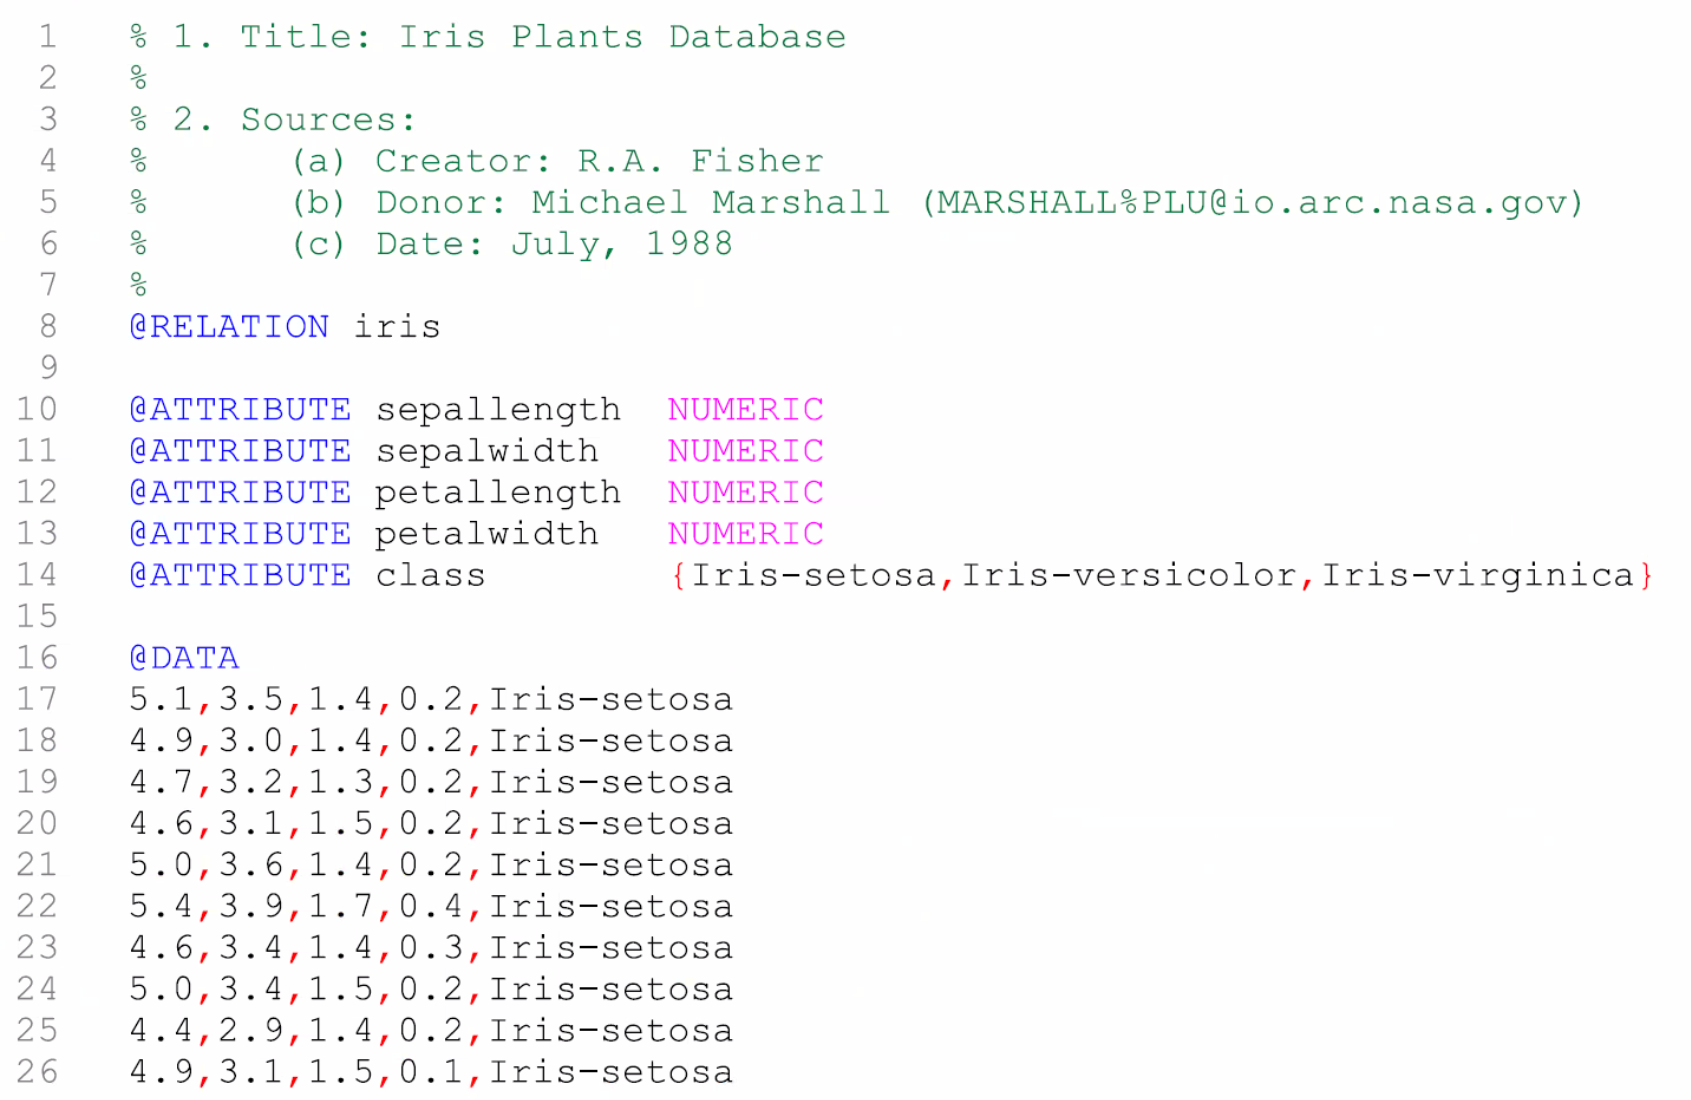
\includegraphics[width=0.9\linewidth]{Images/ARFF-example}
        \label{fig:arff-example}
    \end{figure}\noindent
    Прочие типы данных.
    \begin{itemize}
        \item Картинка. Самое простое~--- двух- (или трёх-)мерная матрица. И есть 1000 алгоритмов, как привести её в один вектор (притом довольно маленький).
        \item Текст. Тут сложнее. Самое тупое~--- посчитать частоту слов. Но не надо, тут сразу двигайте в сторону LLM.
        \item Звук. Это сигнал во времени, и самый простой вариант его представить~--- вектор значений. Для него тоже есть всякие штуки типа спектрограммы Мэла, чтобы преобразовывать звук во что-то более адекватное.
        \item Видео. Это мультимодальный объект, то есть объект, в котором разные типы внутри. Их анализировать тоже своими методами.
    \end{itemize}
    \paragraph{Нормализация.} Зачем? Чтобы признаки с большей дисперсией не влияли на результат сильнее остальных.\\
    Как? Сначала отбросим единицы измерения. Чтобы это было корректно, алгоритм должен быть инвариантен относительно линейных преобразований над признаками. А дальше надо как-то нормализовать дисперсию. Можно, например, вычесть из каждого признака минимум и поделить на разность между максимумом и минимумом. Это $[0;1]$-масштабирование. А ещё можно вычесть (выборное) мат. ожидание из признака и поделить на (выборное) стандартное отклонение это Z-масштабирование. Способов ещё куча, но это два простых.\\
    Как жить с ситуацией, когда у нас признаки зависимы? Никак не жить, если так, вы плохо собрали данные.
    \paragraph{Веса и сэмплирование.}
    Отлично, мы всё нормализовали, а теперь у нас из специфики задачи какие-то признаки более важны. Или могут быть объекты более важны.\\
    Говорят, что объект/признак обладает весом $w$, если он в $w$ раз больше влияет на результат. Если $w$ целое, то это эквивалентно тому, что объект/признак встречается $w$ раз.\\
    Примеры: учёт веса признака
    \[
    \operatorname{dist}(a;b)=\sqrt{\sum\limits_{j=1}^mw_j(a_j-b_j)^2}
    \]
    учёт веса объекта:
    \[
    \mathfrak L_D(\theta)=\sum\limits_{x\in D}w(x)\mathfrak L(x;\theta)
    \]
    А есть сэмплирование: вместо вхождения кучу раз в датасет мы можем сэмплировать объекты с вероятностью $\frac{w_j}{\sum w_j}$.\\
    Ещё это может использоваться для балансировки. Если вы знаете, что реальное распределение не очень сочетается с распределением данных, то мы можем пореже выбирать объекты мажоритарного класса или почаще объекты миноритарного класса (например, в данных одна группа большая, а другая~--- маленькая, а в жизни они равны, и мы даём большие веса малой группе). Да и в принципе, если нас не интересует распределение признаков по классам, распределение будет чаще подсовывать вам штуки из мажоритарного класса, что вам не всегда хочется.\\
    Как сэмплировать? Можно рандомно, можно каждый $x$-тый объект (систематически), можно стратифицированно (ровно в соотношение с какой-то категорией), можно кластерное (если кто-то уже за нас разбил объекты на множества, их множеств можно выбрать несколько).
    \paragraph{Шум.}
    Аномалии~--- плохие объекты для модели. Ошибки~--- плохие объекты для реальности. Пример: пусть у нас есть расход топлива автомобилями. И у нас у одного указан 30л / 100км. Если это грузовой автомобиль, а остальные~--- легковые, то это аномалия. А если объект всем хорош, и данные такие, то это ошибка (а возникнуть такое могло из-за того, что кто-то подразумевал мили на галлон).\\
    Пропуски в наборе данных. Откуда? Из склейки разных наборов данных, из изначально херовых данных или откуда угодно ещё. В CSV нет стандартного способа это обозначить, в ARFF это вопросик, а ещё можно специальное значения: None/Null для строк, категория с несуществующим номером для категорий или NaN для числа. Что делать с этим? Вырезать (признак или объект), заменить (заполнить пропуск средним арифметическим/модой/алгоритмом предсказания, который умеет в пропуски) или добавить (добавить новый признак, который говорит, были ли пропуск или нет; если там была категория, можно отдельное значение категории туда добавить, а не новое свойство делать).
    \\\\\\
    \section{Терминология.}
    \paragraph{Виды искусственного интеллекта.}
    \begin{itemize}
        \item \textbf{Слабый (узкий) ИИ}. Нацелен на решение специфичной задачи, причем способ ее решения не подходит для решения других задач.
        \item \textbf{Сильный (общий) ИИ}. Способен решать множество задач, достигает или превосходит человеческие способности.
        \item \textbf{AI-полная задача}~--- задача, решение которой предполагает создание сильного AI.
        \item \textbf{Проблема ускользающей цели}~--- по мере решения задач ИИ их выписывают из списка задач сильного ИИ и относят к задачам слабого ИИ.
        \item\textbf{Интеллектуальная система}~--- система, решающая одну или несколько задач ИИ.
        \item Помимо машинного обучения выделяют \textbf{экспертную систему}, построенную на основе фактов и правил, извлекаемых из экспертов.
    \end{itemize}
    Отличия экспертной системы от ML:
    \begin{itemize}
        \item Экспертная система строится не от частного к общему, как ML, а от общего к частному.
        \item Экспертная система получает решение не с помощью обучения на большом количестве данных, а с помощью привлечения экспертов (лингвистов) для формализации правил и выстраивания паттернов.
    \end{itemize}
    \paragraph{Связь ML и других дисциплин..}
    \underline{Статистика.} Цель статистики~--- на основе большого числа данных выявить паттерны, по которым строятся эти данные (т.е. распределения и другое). ML не всегда основано на статистике, но часто является <<\textit{более сильной версией}>> статистики.\\
    \underline{Анализ данных.} Пока ML~--- разработка алгоритмов, DA~--- это их применение.
    \paragraph{Устройство машинного обучения глобально.}
    Определение 1: машинное обучение~--- процесс, дающий компьютерам способность обучаться новому, не будучи непосредственно запрограммированными делать это.\\
    Определение 2: программа обучается с опытом $E$ решению некоторой задачи $T$, по метрике качества $P$, если качество ее решения задачи $T$, измеренное согласно $P$, растет вместе с увеличением $E$.\\
    Задача машинного обучения состоит из:
    \begin{itemize}
        \item Набора данных $\mathcal{D}$.
        \item Целевой функции~--- либо функция качества (выигрыша, правдоподобия) $\mathcal{Q}$, либо функция потерь (ошибок, риска) $\mathcal{L}$.
    \end{itemize}
    Алгоритм учится решать задачу, если он максимизирует функцию качества (или минимизирует функцию потерь) для заданного набора данных ($\mathcal Q_{\mathcal D}$ или $\mathcal L_{\mathcal D}$ соотвественно).\\
    В задачах оптимизации у нас есть некая функция потерь $\mathcal{L}$, для которой мы хотим найти минимум, то есть такой вектор параметров $\theta$, что $\mathcal{L}(\theta)\rightarrow\min$. В задачах машинного обучения помимо параметров есть еще данные. Если мы поменяем датасет, минимум функции тоже поменяется. Чтобы их учесть, давайте на каждом объекте набора данных измерим функцию потерь для этого объекта с конкретными параметрами и будем минимизировать сумму этих значений по всем объектам:
    \[\mathcal{L}_{\mathcal{D}}(\theta)=\sum_{x\in\mathcal{D}}\mathcal{L}(x, \theta)\rightarrow\min\]
    Эту сумму можно было бы поделить на размер набора данных, но поскольку он всегда константный вне зависимости от $\theta$, можно минимизировать без него.
    \paragraph{Аппроксимация функции ошибки.}
    Иногда функция качества или функция потерь, которую сообщает заказчик, не формализуется или слишком сложно вычислима. В таком случае выбирается другая функция, которая определяется конкретной задачей машинного обучения. Почему так норм? Ну, например, потому, что настоящая функция потерь уже наверняка была упрощена при формализации потери. Или потому, что при подсчёте истинной функции потерь мы будем работать непростительно долго.\\
    Аппроксимация применяется не только по отношению к функциям: например, в реальной жизни данных может быть потенциально бесконечное количество, но в задаче мы ограничиваемся конечным набором (выборкой).
    \paragraph{Алгоритм машинного обучения в деталях.}
    Обычно у алгоритмов в жизни есть параметры и ввод. И исходя из них алгоритм выдаёт какой-то вывод. Например, утилите \Verb|ffmpeg| вы скармливаете видеофайл(ы) и опции вида \Verb|-b:v|, \Verb|-b:a| и любые другие. А она вам выдаёт какие-то другие видеофайл(ы). Тут ситуация несколько другая:
    \begin{figure}[H]
        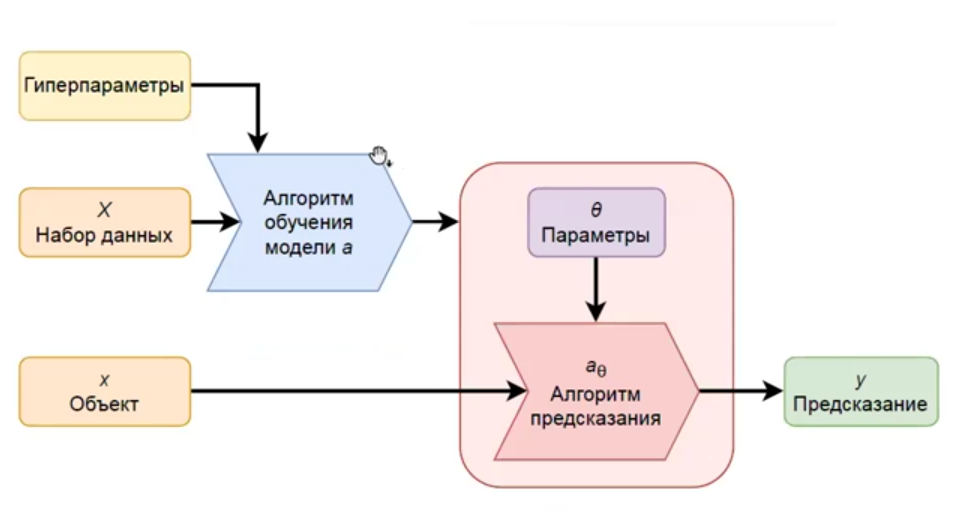
\includegraphics[width=0.8\linewidth]{Images/ml_scheme.png}
        \label{img:ml_scheme}
    \end{figure}\noindent
    Мы хотим сделать алгоритм предсказания, который по объекту делает предсказания. Но тут у нас параметры нам даёт не пользователь, а мы делаем их сами. А точнее, пишем специальный алгоритм (алгоритм обучения), который их нам и сделает. И это уже обычный алгоритм, с обычным входом и выходом. Его вход~--- набор данных, его выход~--- параметры алгоритма предсказания, а его параметры называются специальным словом <<\textbf{гиперпараметры}>>. То есть параметры~--- это параметры модели, которые меняются в процессе обучения, а гиперпараметры~--- фиксированные параметры алгоритма обучения.\\
    Пример: аппроксимация полиномом. Мы решили, что наш алгоритм предсказания будет выглядеть как
    \[
    y=a+bx+cx^2+dx^3+\cdots
    \]
    Где $x$~--- вход, $y$~--- выход, а $a,b,c,d,\ldots$~--- параметры. И для обучения мы себе выбрали, что будем искать только полиномы размерности 2. Тогда вот это вот <<2>>~--- гиперпараметр, точки~--- набор данных, а $a,b,c,0,0,\ldots$ будут нашими параметрами.
    \subparagraph{Уровни модельности алгоритмов.}
    \begin{enumerate}
        \item \textbf{Безмодельные алгоритмы} (<<in-place>>) решают задачу без явного построения модели. Самый тупой пример~--- нахождение матожидания и использование его как результат всех предсказаний. То есть in-place алгоритм не имеет обучения и параметров, он просто запоминает данные и гиперпараметры, и сразу на основе них делает предсказание.
        \item \textbf{Моделирующие алгоритмы} обучаются один раз и строят модель, которую потом можно переиспользовать без повторного обучения, но нельзя обновить при поступлении новых данных. Пример~--- алгоритмы кластеризации.
        \item \textbf{Алгоритмы онлайн-обучения} имеют возможность переобучаться при добавлении новых данных.
        \item Возможность объединить две модели.
    \end{enumerate}
    \paragraph{Определение понятий машинного обучения.}
    Непонятно, что называть решением задачи машинного обучения: алгоритм обучения модели, обученную модель или результат ее применения? Также непонятно, от чего вычисляется функция оценки качества: от алгоритма, от модели или от ее применения. Ответ: зависит от ситуации. Обозначим за $A$ алгоритм обучения, за $\theta$~--- полученные в результате обучения параметры, за $a_{\theta}$~--- полученную в результате обучения модель с параметрами $\theta$. Введем следующие функции оценки качества:
    \begin{enumerate}
        \item $\mathcal{L}(A,\mathcal{D})$~--- функция от алгоритма обучения
        \item $\mathcal{L}_{\mathcal{D}}(a_{\theta})$~--- функция от обученной модели
        \item $\mathcal{L}(\widehat{y},y)$, $\widehat{y}=a_{\theta}(x)$~--- функция для результата применения, то есть отклонение истинного результата от предсказанного обученной моделью
    \end{enumerate}
    Очевидно, нам хочется, имея одну из этих функций, вычислять остальные. Поэтому введем три понятия:
    \begin{enumerate}
        \item \textbf{Валидация}~--- вычисление $\mathcal{L}(A,\mathcal{D})$ из $\mathcal{L}_{\mathcal{D}}(a_{\theta})$.
        \item \textbf{Тестирование модели} $a_{\theta}$ на наборе данных $\mathcal{D}$~--- вычисление $\mathcal{L}_{\mathcal{D}}(a_{\theta})$ из $\mathcal{L}(\widehat{y},y)$.
        \item \textbf{Применение}~--- вычисление $a_{\theta}(x)$.
    \end{enumerate}
    \subparagraph{Валидация на отложенных данных.}
    Пусть мы хотим понять обобщающую способность нашей модели, но у нас есть ограниченный набор данных. Мы хотим убедиться, что наша модель будет выдавать хорошие результаты за пределами датасета, на котором ее обучали (для этого мы ее и обучаем). Обычно в таких случаях исходный датасет разбивают на training и test часть случайным образом. (Вообще, необязательно случайным; например, если объекты могут составить временной ряд, то разбивать объекты лучше по времени.) Тогда:
    \[\mathcal{L}(A,\mathcal{D})=\mathcal{L}(A(\mathcal{D}_{\mathrm{train}}),\mathcal{D}_{\mathrm{test}})\]
    \paragraph{Сравнение алгоритмов.}
    Чтобы сравнить в машинном обучении два алгоритма, один из которых не является частным случаем другого (тогда очевидно, что общий алгоритм лучше), нужно, во-первых, ввести метрику их сравнения, а во-вторых сравнивать на одинаковых наборах данных. Под метрикой подразумевается уже знакомая нам функция качества от алгоритма $\mathcal{L}(A,\mathcal{D})$, а также способ ее вычисления. Часто при решении задачи берут какой-то наивный алгоритм (baseline) и сравнивают остальные алгоритмы с ним. Теорема <<No free lunch theorem>> гласит, что алгоритм может работать хорошо только на определенном наборе данных, а на остальных данных проседает, т.е. нельзя покрыть одним алгоритмом все, нужно выбирать исходя набора данных в данной задаче. Лучший алгоритм для конкретной задачи с конкретным набором данных и конкретной метрикой называется State-of-the-art (SOTA).
    \paragraph{Стандартные задачи машинного обучения.}
    \begin{figure}[H]
        \begin{tabularx}{0.8\textwidth}{|X|XXX|}
            \hline
            $a\colon X\to Y$ & $Y=\{y_1,\ldots,y_k\}$ & $Y=\operatorname{Pr}^k$ & $Y=\mathbb R^k$\\
            \hline
            Обучение с учителем & Классификация & Мягкая классификация & Восстановление регрессии\\
            \hline
            One-class classification & Поиск аномалий & Восстановление плотности & {\color{red}Генерация объектов}\\
            \hline
            Обучение без учителя & Кластеризация & Мягкая кластеризация & Выделение признаков\\
            \hline
        \end{tabularx}
    \end{figure}\noindent
    Что здесь происходит? Задачу машинного обучения можно представить как отображение из $X$ в $Y$.
    В качестве столбцов у нас то, что может быть результатом:
    \begin{itemize}
        \item $Y=\{c_1,c_2,...,c_n\}$: результатом является сопоставление класса каждому объекту из набора. 
        \item $Y=\operatorname{Pr}^k$: результатом является сопоставление вектора вероятностей размера $k$ каждому объекту из набора.
        \item $Y=\mathbb{R}^k$: результатом является одно число или вектор чисел размера $k$.
    \end{itemize}
    В качестве строк выступает то, что служит источником для построения модели:
    \subparagraph{Обучение с учителем}
    В качестве источника выступают размеченные данные, то есть выборка, содержащая верные ответы. Цель алгоритма~--- научится эти правильные ответы предсказывать.
    \begin{itemize}
        \item \textbf{Задача классификации}~--- задача сопоставления каждому объекту категории на основе распределения по категориям в обучающем датасете. Наивное решение~--- всегда брать моду (самый популярный класс). Примеры: определить, является и письмо спамом или определить, какая цифра на картинке.
        \item \textbf{Задача мягкой классификации}~--- задача сопоставления объекту вектора, где каждое число обозначает уверенность в попадании объекта в конкретный класс. Выделяют вероятностную классификацию, где вектор должен быть корректным вероятностным вектором.
        \item \textbf{Задача восстановления регрессии}~--- задача предсказания ответа для произвольного объекта на основе сопоставления ответов объектам в обучающем датасете. Наивное решение~--- брать мат. ожидание.
    \end{itemize}
    Ещё в случае обучения с учителем $Y$ может быть перестановкой или рангом. В таком случае мы пытается установить порядок на наших объектах. Используется это крайне редко.\\
    Особняком стоят задачи прогнозирования временных рядов, где при имеющихся $y_{t-m},\ldots,y_{t-2},y_{t-1}$ надо предсказать $y_t$. Самый яркий пример~--- цены акций. Особняком они потому, что у них нет признаков (кроме, собственно, $y_t$). Где такие взять? Ну, например, считать, что
    \[
    x_t=(y_{t-m},\ldots,y_{t-2},y_{t-1})
    \]
    Это называется авторегрессия. Или можно брать какую-то функцию от $t$, это конструирование признаков. Наивное решение~--- арифметическое скользящее среднее или экспоненциально скользящее среднее.
    \begin{figure}[H]
        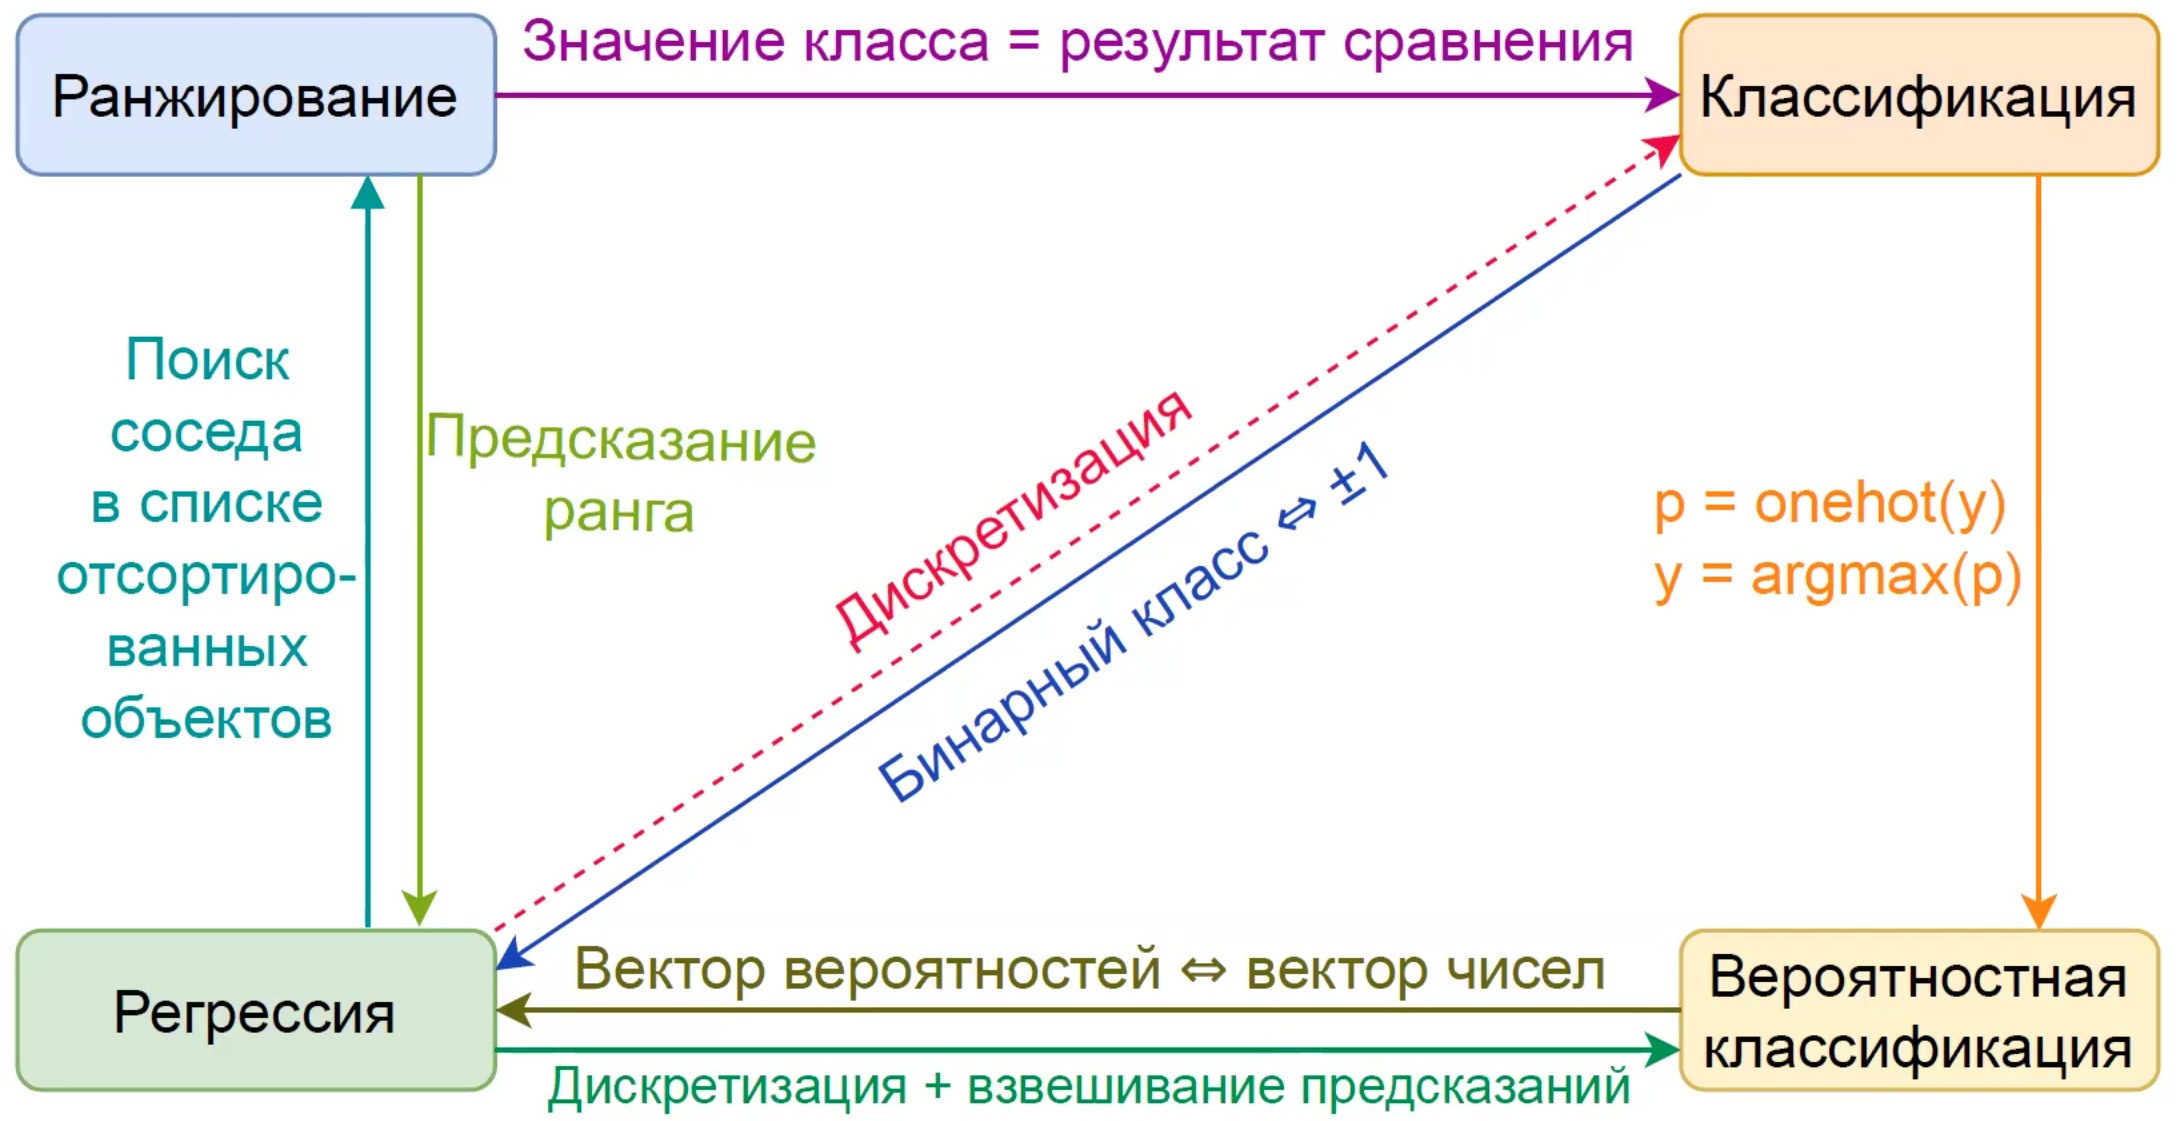
\includegraphics[width=0.8\linewidth]{Images/Supervised-learning-problem-convertions}
    \end{figure}\noindent
    \subparagraph{One-class classification}
    В качестве источника выступают данные, почти все из которых принадлежит одному классу (известно для каждого объекта, принадлежит он или нет).
    \begin{itemize}
        \item \textbf{Задача поиска аномалий}~--- среди существующих объектов нужно найти объекты другого класса.
        \item \textbf{Задача новизны}~--- среди каких-то новых объектов нужно найти объекты другого класса.
        \item \textbf{Задача восстановления плотности}~--- требуется восстановить плотность распределения и для новых объектов определить, кто из них выбивается из распределения. Обычно используется метод максимального правдоподобия, где мы оцениваем параметры распределения на основе объектов из выборки. Подробнее~--- на матстате.
        \item \textbf{Задача генерации новых объектов}~--- по данным объектам нужно сгенерировать новые.
    \end{itemize}
    Не путайте генерацию с сэмплированием (выбрать объект из существующих) и аугментацией (примитивными аналитическими операциями сгенерировать новые объекты, например, повернуть картинку котика, чтобы получить новую картинку котика). Это другие вещи, но их можно использовать как наивное решение.\\
    Из интересного, чтобы оценить качество генерации используются алгоритмы классификации (на два класса: реальный объект или сгенерированный). А ещё можно сохранять некоторую статистику между реальными объектами, тогда классификация разделяется на два вида моделей:
    \begin{itemize}
        \item Генеративные~--- обучают совместное распределение вероятностей, и задача классификации сводится к задаче восстановления плотности.
        \item Дискриминативные~--- обучают условное распределение, и модель пытается найти разделяющее правило.
    \end{itemize}
    Обычно используются в паре, но об этом подробнее во втором семестре.
    \subparagraph{Обучение без учителя.}
    В качестве источника выступают неразмеченные данные, для которых требуется самостоятельно придумать целевой признак $\widehat Y$. И дальше уже распределение на задачи ведётся в зависимости от того, каким является наш $\widehat Y$ (а не $Y$, как было в таблице).
    \begin{itemize}
        \item \textbf{Задача кластеризации}~--- требуется разделить объекты на подмножества (кластеры), чтобы в каждом кластере объекты были максимально похожи друг на друга. Пример: вы пишете Твиттер, и хотите разделить пользователей по информационным пузырям.
        \item \textbf{Задача мягкой кластеризации}~--- аналогично мягкой классификации.
        \item \textbf{Задача выделения признаков}~--- алгоритм должен отображать объект из $X$ в пространство (чаще всего меньшей размерности), которое он сам и придумает. Самое наивное~--- умножим на рандомную матрицу. Используется для уменьшения размерности, чтобы, например, нарисовать наши данные.
        \item \textbf{Задача конструирования признаков}~--- по сути, более общая задача извлечения признаков: дана какая-то абстрактная штука (картинка, текст, etc), хочется сделать себе вектор признаков. Решается явно, а не алгоритмами ML. Пример: пытаемся наложить шаблон на изображения, суммируем по всем возможным наложениям. Получаем новый признак для каждого шаблона. А вот шаблоны уже можно искать машинным обучением.
    \end{itemize}
    \subparagraph{Другие задачи машинного обучения.}
    \begin{itemize}
        \item Можно не только принимать на вход пропуски, но и возвращать. Трактуется как отказ от классификации/кластеризации. Первое используется в ансамблях, второе~--- в поиске аномалий.
        \item \textbf{Предсказание и заполнение пропусков}. Выберем признак с пропусками целевым, остальные заполним как-нибудь, натренируем модель на данных без пропусков, заполним пропуски результатом тестового прогона.
        \item \textbf{Коллаборативная фильтрация}. Дано множество оценок пользователями. И оценок, блин, мало (существенно меньше произведения числа пользователей и вещей). Требуется предсказать оценку данной вещи данным пользователем. Решается трудно, этим занимается специальный раздел (рекомендательные системы), очевидно, тем же алгоритмом, что заполнение пропусков, оно не решается, зато наоборот (заполнить пропуски совместной фильтрацией)~--- норм план.
        \item \textbf{Обучение на привилегированных данных}. Тренировочные данные содержат дополнительную информацию ($X'$), недоступную при тестировании. Базовое решение: либо не использовать $X'$, либо взять другую модель, которая предсказывает $X'$, и пользоваться ей, либо честно самому предсказывать и $X'$, и $Y$. Пример: предсказываем результат футбольного матча, и наши привилегированные данные~--- число красных и жёлтых карточек, например. На тестовых данных такое неизвестно.
        \item \textbf{Обучение на частично размеченных данных} (оно же \textbf{обучение с частичным привлечением учителя}). Лишь малая часть тренировочных данных (и никакая часть тестовые данные) содержит правильный ответ. Наивное решение: не использовать разметку (т.е. обучаться полностью без учителя) или не использовать неразмеченные объекты.
        \item \textbf{Активное обучение}~--- вариация на тему предыдущего. Можно задавать Оракулу вопросы о значении меток, и надо за минимум обращений к Оракулу восстановив $f\colon X\to Y$. То есть по сути надо не функцию найти даже, а стратегию выработать, как обращаться к Оракулу.
        \item Обучение с подкреплением (Reinforcement Learning). Есть агент и есть среда. Агент взаимодействует со средой, среда меняет состояние и возвращает награду. Задача: максимизировать награду. Пример: задача об одноруком бандите, он что-то знает об одноруком бандите, и должен выработать стратегию, как максимизировать выигрыш.
    \end{itemize}
    \section{Обучение с учителем.}
    Если алгоритм работает хуже или сравнимо с наивным (наивный, напомню, берёт моду / мат. ожидание меток), значит или алгоритм плох (и не выявляет зависимость $Y$ от $X$), либо данные плохи (и в них $Y$ не зависит от $X$).\\
    Сведение к бинарной классификации: пусть у нас есть алгоритм бинарной вероятностной классификации. Как из него многоклассовую сделать?
    \begin{itemize}
        \item <<Один против всех>>. Заданный класс помечаем как единицу, остальные~--- как минус единицу. Возьмём $k$ таких классификаторов, у кого вероятность больше, того и берём.
        \item <<Один против одного>>: обучим $\frac{k(k-1)}2$ классификаторов $a^b_{u,v}$: для каждой пары классов $u,v$ выберем множество объектов $X_{u,v}$, принадлежащих одному из этих классов. Обучим на этом множестве классификатор $a^b_{u,v}$ предсказывать вероятность того, что объект принадлежит $u$, после чего сделаем себе
        \[
        a(x)=\operatorname*{argmax}_c\prod\limits_va^b_{c,v}(x)\cdot\prod\limits_u(1-a^b_{u,c}(x))
        \]
        Тут обучаем много классификаторов, но для каждого выборки поменьше.
    \end{itemize}
    На мягкой классификации тоже работает.
    \paragraph{Настройка гиперпараметров как часть обучения.}
    Помните \hyperref[img:ml_scheme]{красивую идеалистичную картинку} про гиперпараметры, параметры и данные? Так вот на самом деле ситуация иная:
    \begin{figure}[H]
        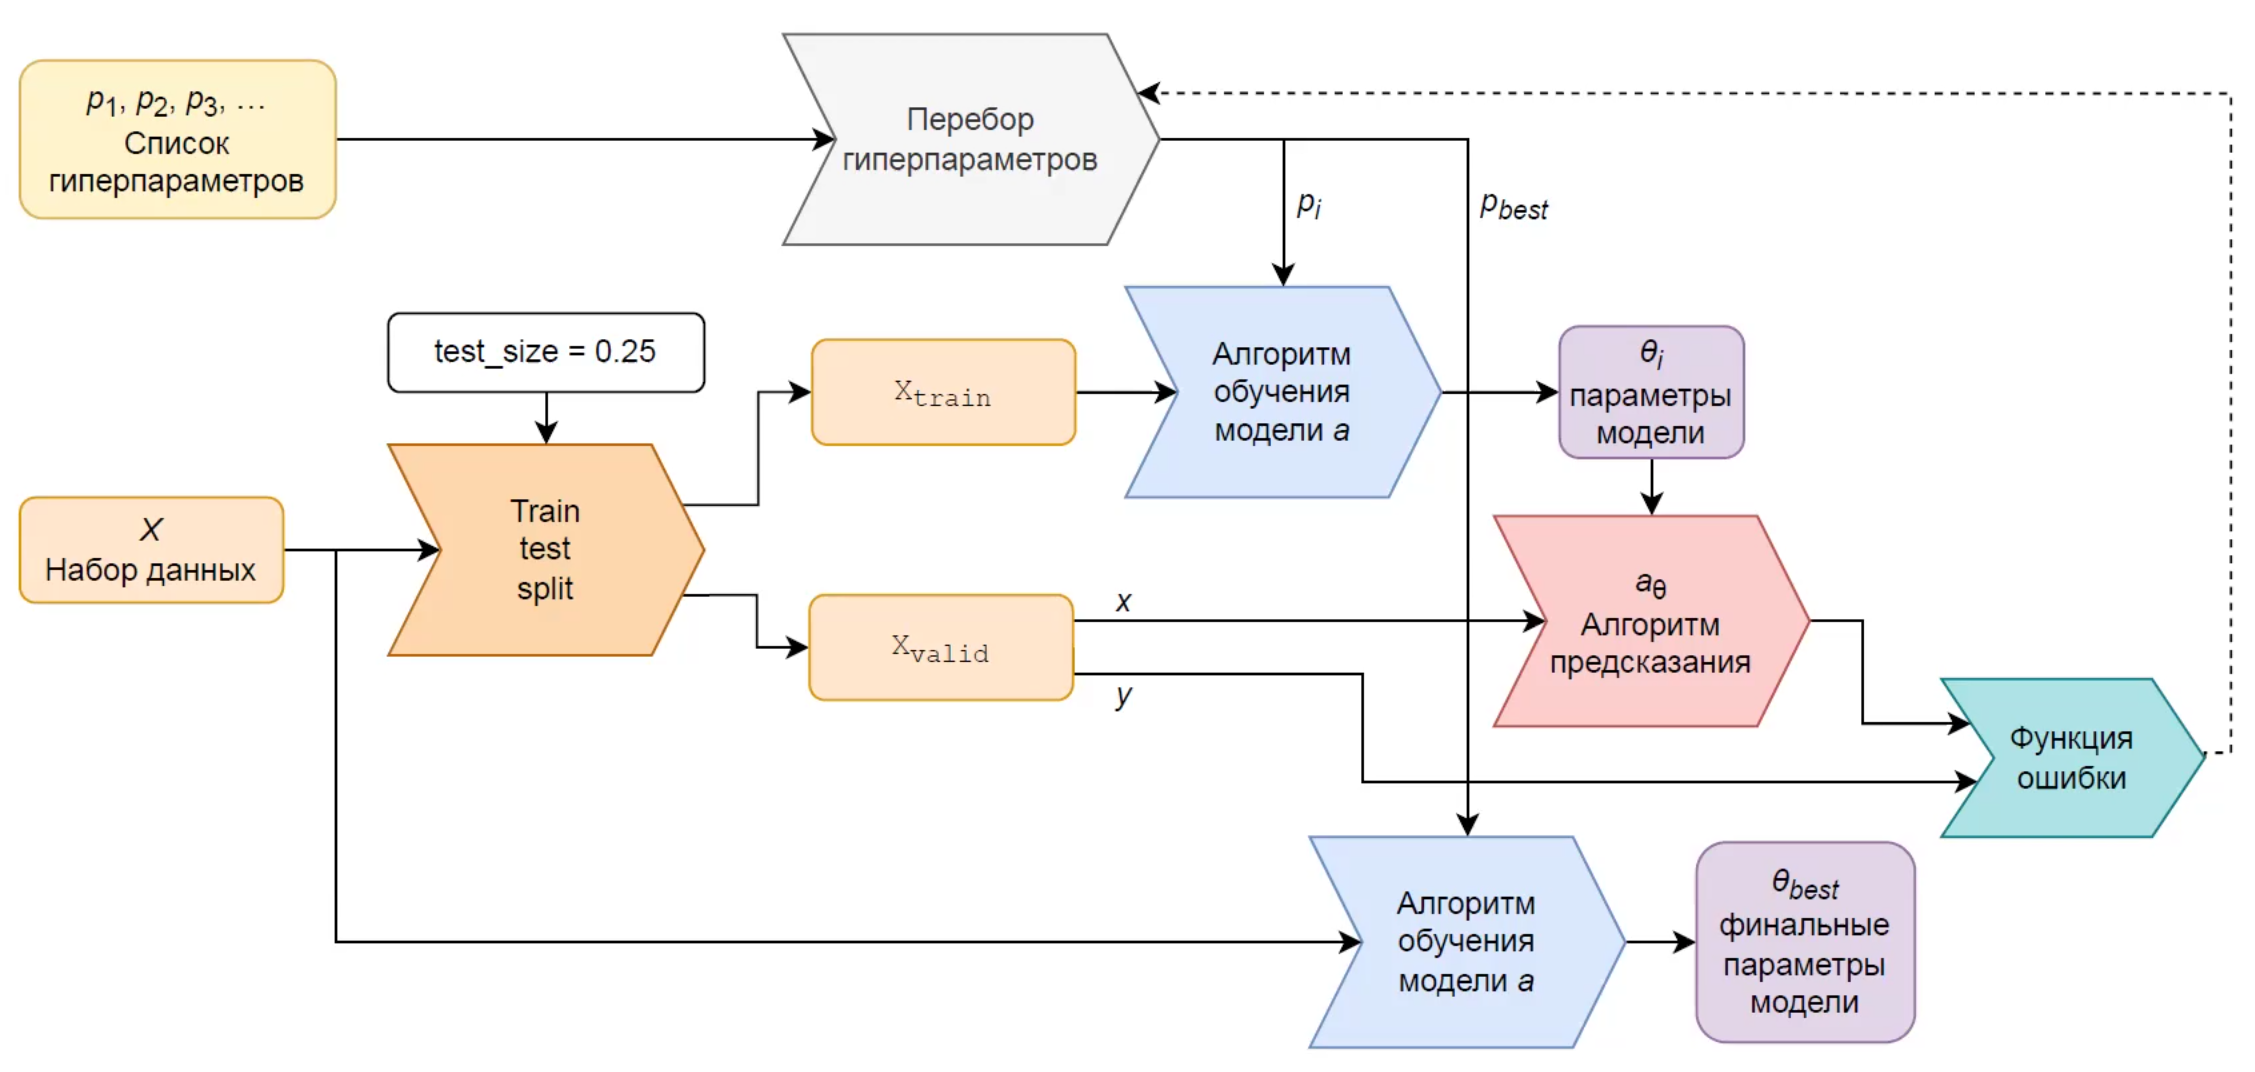
\includegraphics[width=0.8\textwidth]{Images/ml_scheme_advanced}
    \end{figure}\noindent
    Естественно, гиперпараметры тоже надо настраивать, и не руками. Делим нашу выборку на две части: $X_{\mathrm{train}}$ и $X_{\mathrm{valid}}$. И гиперпараметры у нас не одни, а несколько комбинаций. Мы кидаем этот набор в некоторый алгоритм перебора гиперпараметров, он нам даёт какие-то гиперпараметры, кидаем его в обучение, из них и $X_{\mathrm{train}}$ получаем параметры. Дальше из алгоритма предсказания и $X_{\mathrm{valid}}$ получаем функцию ошибки. Из неё меняем гиперпараметры. Повторим до тех пор, пока всё не будет хорошо. Когда будет~--- засунем уже весь набор в обучение и получим финальные параметры модели.\\
    $X_{\mathrm{valid}}$ называется \textbf{валидационным множеством}. Иногда финальные параметры модели не берут заново, а берут ровно последний получившийся из обучения на $X_{\mathrm{train}}$ алгоритм. Ещё из интересного алгоритм обучения обычно неявно настраивает гиперпараметры (если может это сделать). Например, градиационный спуск имеет гиперпараметром количество шагов, но он итеративный алгоритм, и он сам примерно знает, когда его останавливать.\\
    \textbf{Начальное состояние генератора псевдослучайных чисел нельзя настраивать!}\\
    Как настраивать гиперпараметры? Поиск по сетке, случайный поиск эволюционные алгоритмы, или, из современного, байесовская оптимизация.
    \paragraph{Переобучение и регуляризация.}
    Начиная с определённого уровня сложности модели, чем лучше он работает на тренировочных данных, тем хуже на реальных. Пример: у нас есть $y(x)=\frac1{1+25x^2}$. Мы не знаем $y$. И мы аппроксимируем это чудо полиномом. Притом всё делаем на $[-2;2]$. Тогда где-то до степени 15 ошибка на контрольной выборке падает, а потом резко начинает расти. Выглядит это примерно так:
    \begin{figure}[H]
        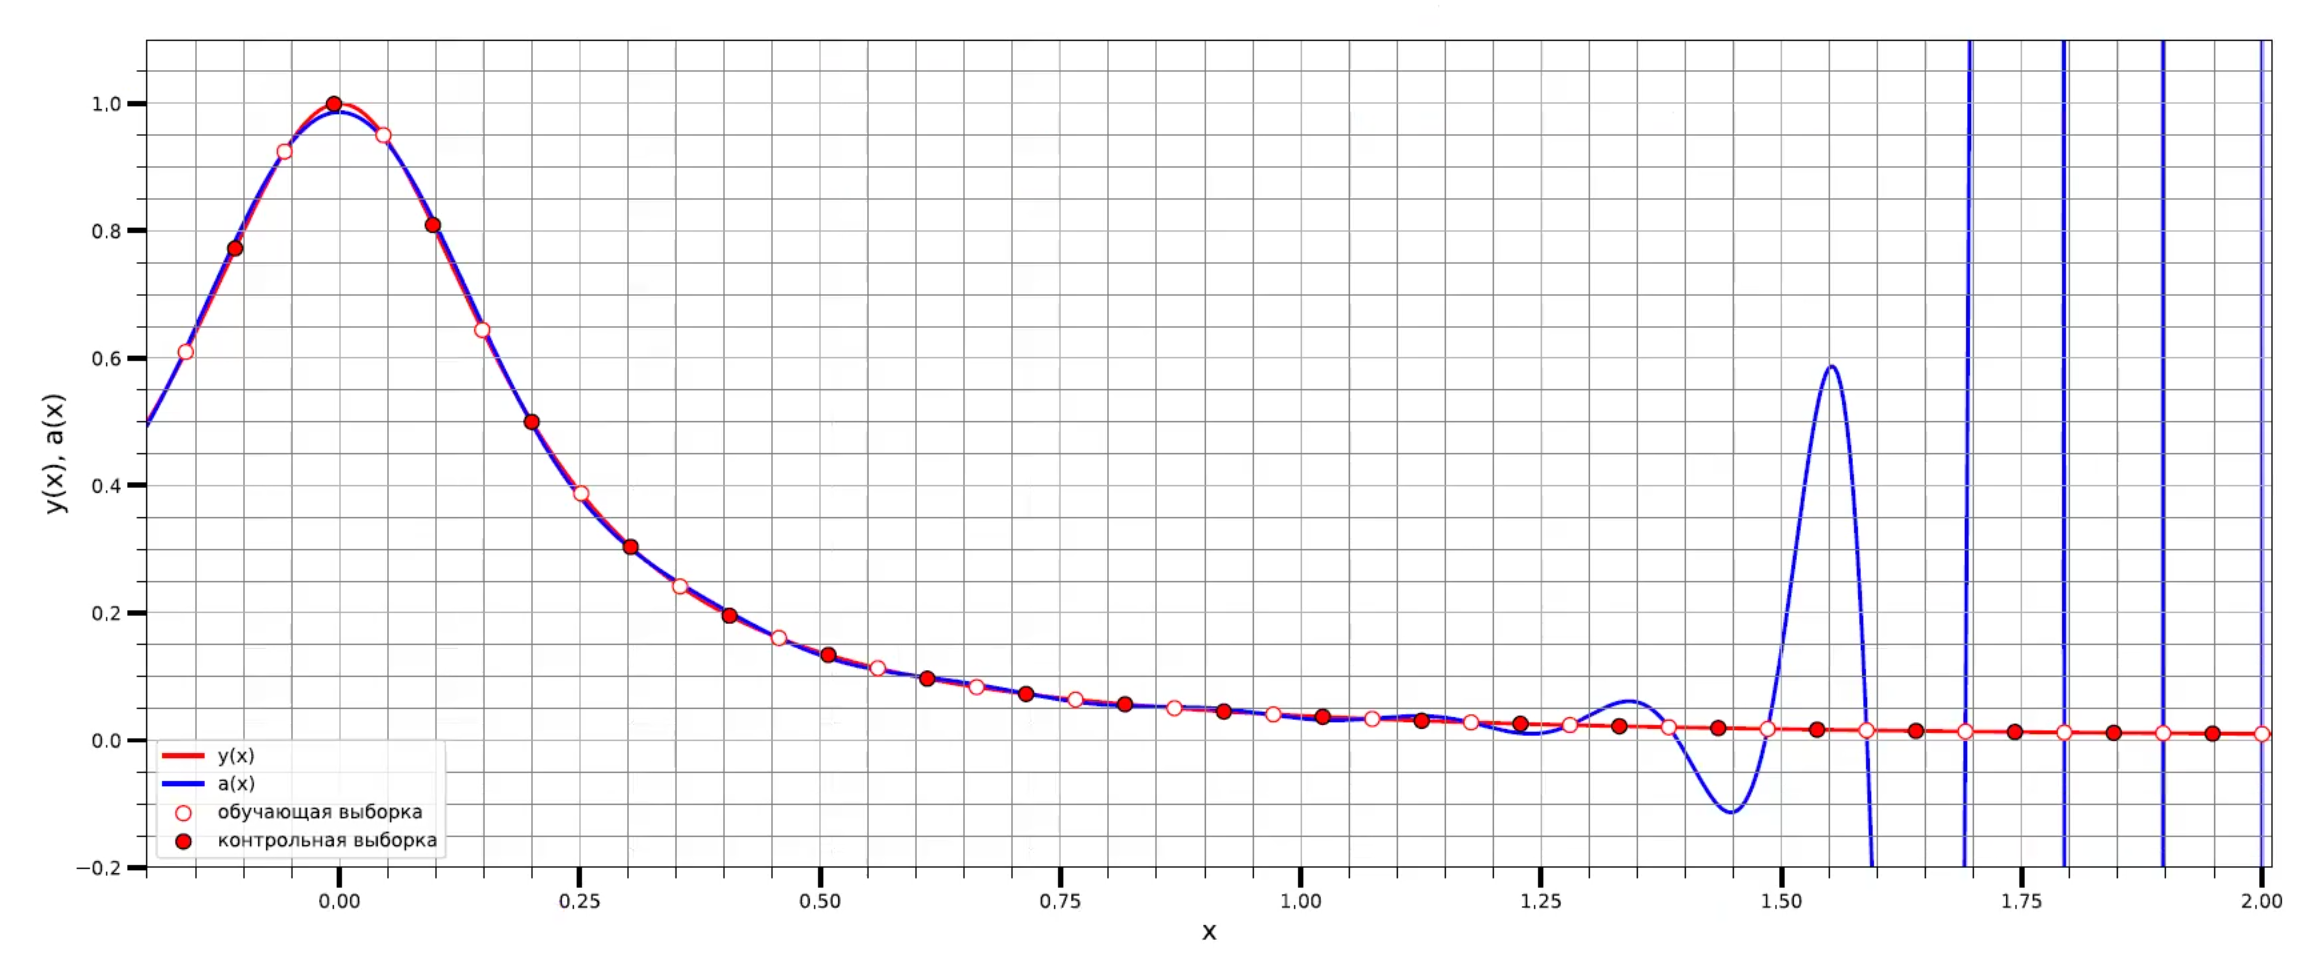
\includegraphics[width=0.8\textwidth]{Images/ml_overfitting_example}
    \end{figure}\noindent
    Тут взята степень где-то 32, белые точки~--- обучающая выборка, красные~--- контрольная. Видно, что ошибка модели на контрольной модели огромна, а на обучающей она примерно ноль.\\
    Аналогично есть недообучение, когда нам просто не хватает сложности модели:
    \begin{figure}[H]
        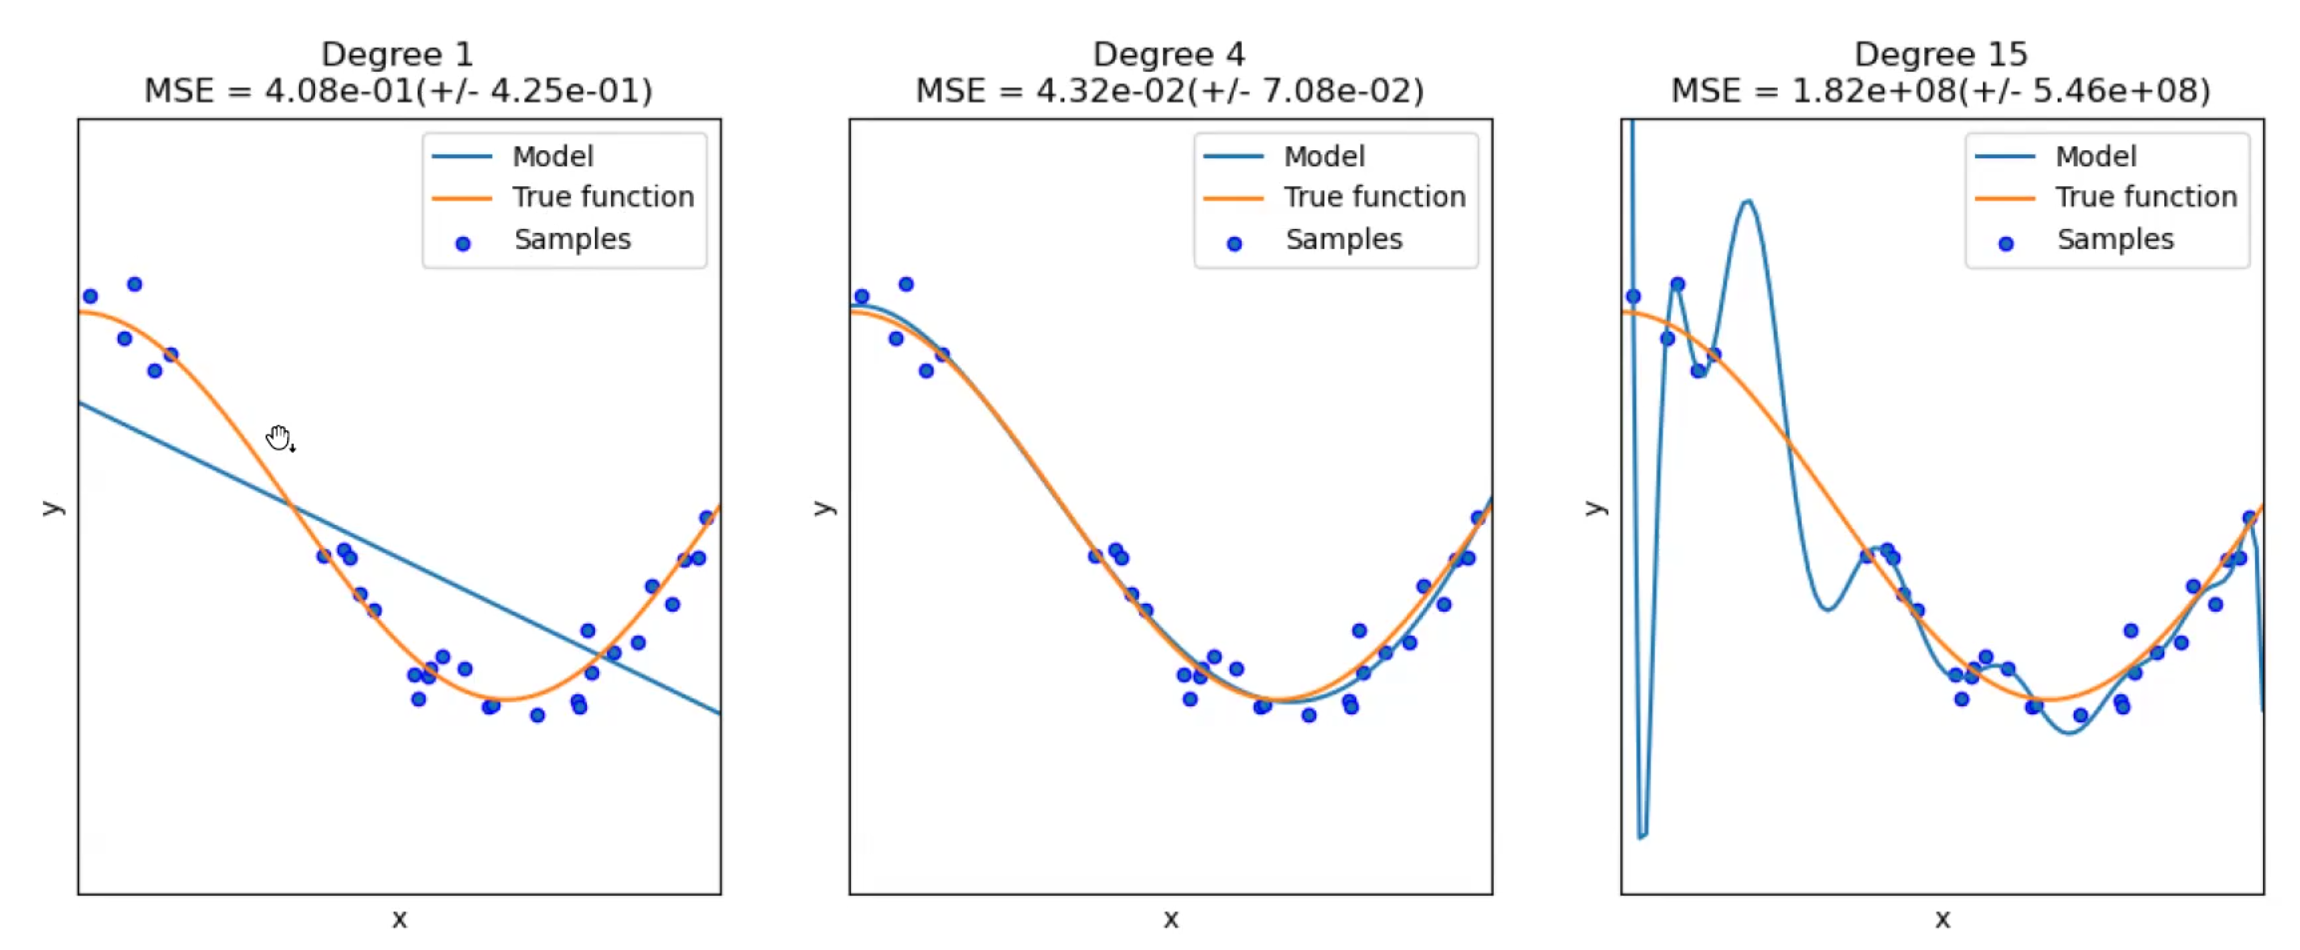
\includegraphics[width=0.8\textwidth]{Images/ml_overfitting_underfitting}
    \end{figure}\noindent
    Тут в качестве ошибки берётся MSE, и показаны значения ошибки для недообученной и переобученной модели.\\
    В реальной жизни такие картиночки мы не построим, придётся бороться как-то иначе. Для этого есть регуляризация. Это добавление ограничений с целью предотвратить переобучение. ПО сути это штраф за сложность модели:
    \[
    \scriptL_{\mathrm{reg}}(\theta,\scriptD)=\scriptL(\theta,\scriptD)+\lambda\cdot\operatorname{complexity}(\theta)
    \]
    Тут $\lambda$~--- константа, и мы минимизируем $\scriptL_{\mathrm{reg}}(\theta,\scriptD)$.\\
    Это мягкая регуляризация, а есть ещё жёсткая: минимизировать $\scriptL(\theta,\scriptD)$ при условии, что $\operatorname{complexity}(\theta)<C$ ($C$~--- новый гиперпараметр, являющийся ограничением на сложность).
    \subparagraph{Статистическое обоснование переобучения.}
    \begin{itemize}
        \item \textbf{Смещение} (bias)~--- погрешность оценки, возникающая в результате ошибочного предположения в алгоритме. Высокое смещене~--- недообучение.
        \item \textbf{Дисперсия} (variance)~--- ошибка чувствительности к малым отклонениям в тренировочным наборе. Высокая дисперсия~--- переобучение.
    \end{itemize}
    Откуда это всё? Пусть $f$~--- реальная зависимость, $\widehat y$~--- предсказание модели, $y=f(x)+\varepsilon$~--- измерение с шумом $\varepsilon$, где $\Expected[\varepsilon]=0$, $\Variance[\varepsilon]=\sigma^2$. Тогда
    \[
    \Expected[y]=f\qquad\Variance[y]=\sigma^2
    \]
    А отсюда ожидание квадрата ошибки:
    \[\begin{split}
        \Expected\left[(y-\widehat y)^2\right]&=\Expected\left[y^2+{\widehat y}^2-2y\widehat y\right]=\\
        &=\Expected\left[y^2\right]+\Expected\left[{\widehat y}^2\right]-\Expected\left[2y\widehat y\right]=\\
        &=\Variance[y]+f^2+\Variance[\widehat y]+\Expected[\widehat y]^2-2f\Expected\left[\widehat y\right]=\\
        &=\Variance[y]+\Variance[\widehat y]+\left(f-\Expected[\widehat y]\right)^2=\\
        &=\sigma^2+\Variance[\widehat y]+\Bias[\widehat y]^2
    \end{split}\]
    То есть тут неустранимая погрешность измерений, дисперсия модели и квадрат смещения модели.
    \subparagraph{Двойной спуск.}
    Не так давно умные люди показали, что с определённой точки ошибка на тестовых данных снова начнёт падать. Нам это полезно, чтобы нейронные сети не переобучались (потому что в них параметров огромное количество, и возникает вопрос, почему они не переобучаются). Кому очень интересно, почитайте Belkin M., Shu, D.J., Ma, S., \& Mandal, S. (2018). Reconciling modern machine learning and the bias-variance trade-off.\\
    Но работает это только для супер-больших моделей, пока мы не пишем нейронки, у нас всё ещё есть классический bias-variance trade-off.
    \paragraph{Перекрёстная проверка.}
    Пусть $|\scriptD_{\mathrm{train}}|=r$, $|\scriptD_{\mathrm{test}}|=e$. Разобьём наш набор данных всеми возможными способами на $\scriptD_{\mathrm{train}}$ и $\scriptD_{\mathrm{test}}$. Тогда хотелось бы в качестве валидации использовать
    \[
    \scriptL(A,\scriptD)=\frac1{\binom{e+r}e}\sum\limits_{\scriptD=\scriptD_{\mathrm{train}}\cup\scriptD_{\mathrm{test}}}\scriptL(A(\scriptD_{\mathrm{train}}),\scriptD_{\mathrm{test}})
    \]
    Тут мы точно не потеряем обобщающую способность. Но тут нам надо построить и обучить огромное количество моделей, поэтому такой подход (полная кросс-валидация) не используется.\\
    Вместо этого используют кросс-валидацию по $k$ блокам: распилим наш набор данных на $k$ частей, каждая часть будет тестовой ровно один раз. Модель мы будем строить всего $k$ раз таким образом. $k$ бывает 5 либо 10.\\
    Крайний случай~--- валидация по одному объекту Это полная кросс-валидация, где $e=1$.\\
    Ещё бывает стратифицированная кросс-валидация. Если объекты каких-то классов недостаточно часто встречаются, лучше разбивать на блоки так, чтобы в каждом блоке эта статистика была пропорциональна статистике выборки.\\
    Если у нас задача временного ряда (т.е. ранние блоки дают более плохой результат), то тут среднее по всем разбиениям заменяется на среднее взвешенное среднее с экспоненциально растущими весами блоков.\\
    Важно:
    \begin{itemize}
        \item Усреднять суммой можно только аддитивные функции ошибки/качества.
        \item Для усреднения можно использовать $t$ кросс-валидацию по $k$ блокам (повторить кросс-валидацию по $k$ блокам $t$ раз).
        \item Если кросс-валидация используется для настройки гиперпараметров, модель требуется заново обучить на всём наборе данных.
    \end{itemize}
    \subparagraph{Другие причины переобучения.}
    Перекрёстная проверка не поможет вам в следующих случаях:
    \begin{itemize}
        \item Нерепрезентативные (смещённые) данные.
        \item Плохо подобранная метрика качества измерения алгоритма.
        \item Систематические смещения в методах валидации.
        \item Непонимание скрытых гиперпараметров.
    \end{itemize}
    Короче, если вы продолбались сами или данные отстойные, то вам ничего не поможет.
    \subsection{Оценка задачи классификации.}
    Поскольку с категориями нельзя делать ничего, кроме проверки из на равенство, заведём себе вот такую точность:
    \[
    \operatorname{Accuracy}(y;\widehat y)=\frac1n\sum\limits_{i=1}^n[y_i=\widehat y_i]
    \]
    Где $n$~--- количество объектов в выборке, $y$~--- вектор реальных ответов, а $\widehat y$~--- вектор предсказаний. Но тут есть проблема. Представьте, что у вас 90\% объектов одного класса. И вы получили точность 70\%. Это хорошо? Да ну хз, но, вероятно, нет, и вы переобучаетесь на мажоритарный класс.\\
    \textbf{Коэффициент Каппа Коэна}:
    \[
    \kappa(po,pe)=\frac{po-pe}{1-pe}
    \]
    Где $po$~--- полученная точность, а $pe$~--- точность случайного/наивного алгоритма.\\
    Что использовать функцией ошибки? Например, вот это
    \[
    \operatorname{ErrorRate}(y;\widehat y)=\frac1n\sum\limits_{i=1}^n[y_i\neq\widehat y_i]=1-\operatorname{Accuracy}
    \]
    Но это используют редко, чаще используют что-нибудь, что можно производной ковырять.\\
    Из более интересного: Confusion matrix: в ячейке $CM_{t,c}$ хранится количество объектов класса $t$, которые были приняты нашим алгоритмом за объекты класса $c$.\\
    Простой пример: бинарная классификация. Тогда у нас наша матрица состоит из четырёх ячеек, которые, как несложно догадаться, называются <<True Positive>>, <<True Negative>>, <<False Positive>> (мы посчитали, что positive, а оно нет, type 1 error) и <<False Negative>> (type 2 error). Тут следующие величины:
    \begin{itemize}
        \item Точность (не accuracy, а \textbf{precision}): $\displaystyle\frac{\mathrm{TP}}{\mathrm{TP}+\mathrm{FP}}$.
        \item Полнота (\textbf{recall}): $\displaystyle\frac{\mathrm{TP}}{\mathrm{TP}+\mathrm{FN}}$.
        \item Индекс Жаккара (\textbf{JaccardIndex}): $\displaystyle\frac{\mathrm{TP}}{\mathrm{TP}+\mathrm{FN}+\mathrm{FP}}$.
    \end{itemize}
    Так вот, используют такую штуку, как F-мера:
    \[
    F_\beta=(1+\beta^2)\frac{\mathrm{Precision}\cdot\mathrm{Recall}}{\beta^2\cdot\mathrm{Precision}+\mathrm{Recall}}
    \]
    Например, могут использовать $F_1$.\\
    Как делать F-меру для нескольких классов? Ну, можно делать <<один против всех>>, мы уже учились. То есть у нс для каждого класса $j$ сформировались свои $\mathrm{TP}_j$, $\mathrm{FP}_j$ и $\mathrm{FN}_j$. Тогда
    \begin{itemize}
        \item Можно усреднить $\mathrm{TP}$, $\mathrm{FP}$ и $\mathrm{FN}$, из них посчитать $\mathrm{Precision}$ и $\mathrm{Recall}$. Полученная мера~--- micro-average F-score.
        \item Можно для каждого $j$ посчитать $\mathrm{Precision}_j$ и $\mathrm{Recall}_j$, после чего усреднить уже их. Результат будет другим, и называться будет macro-average F-score.
        \item А можно уже посчитать F-score для каждого класса и её усреднить. Это будет average F-score.
    \end{itemize}
    Лучшей среди них нет. Хороший заказчик сам знает, что ему надо из этого.\\
    Ещё есть вот такая штука:
    \begin{itemize}
        \item \textbf{Чувствительность} (true positive rate, $\mathrm{TPR}$)~--- тупо Recall (т.е. $\frac{\mathrm{TP}}{\mathrm{TP}+\mathrm{FN}}$).
        \item \textbf{Специфичность} (true negative rate, $\mathrm{TNR}$)~--- отношение $\frac{\mathrm{TN}}{\mathrm{TN}+\mathrm{FP}}$.
        \item ROC-кривая~--- зависимость $\mathrm{TPR}$ от $\mathrm{TNR}$.
        \item Площадь под ROC-кривой (AUC ROC)~--- функция качества бинарной классификации.
    \end{itemize}
    Рандомный классификатор имеет тупо прямую линию из $(0;0)$ в $(1;1)$. Идеальный~--- точка $(0;1)$. В многоклассовой классификации используется редко, поэтому говорить об этом не будем.\\
    Как ROC строить? Берём мягкую классификацию. Она для каждого объекта сообщает нам вероятность, что объект принадлежит положительному классу. Так вот что мы делаем? А делаем следующее. Установим карандаш в левый нижний угол, будем перебирать $(p_i;y_i)$ по возрастанию $p_i$. Если $y_i$ положителен, сдвинем карандаш право, если отрицателен~--- то вверх. Получим ломаную, которую если аппроксимировать, получится нормальная ROC-кривая.
    \subsection{Оценка задачи регрессии.}
    Как сделать себе функцию ошибки? Есть сумма квадратов и его друзья:
    \begin{itemize}
        \item Простая и популярная функция:
        \[
        \operatorname{SS}(y;\widehat y)=\|y-\widehat y\|^2_2=\sum\limits_{i=1}^n(y_i-\widehat y_i)^2
        \]
        Легко вычисляется, имеет приятную производную, но некорректно сравнивать результаты для массивов разного размера.
        \item
        \[
        \operatorname{MSE}(y;\widehat y)=\frac1n\operatorname{SS}(y;\widehat y)
        \]
        Жаль, размерность не совпадает с размерностью целевого признака.
        \item Чтобы это починить, берём корень $\operatorname{MSE}$ (получаем $\operatorname{RMSE}$). Но одна проблема всё ещё остаётся: нужен baseline.
        \item Чтобы по чинить и это, вводим:
        \[
        \operatorname{NRMSE}(y;\widehat y)=\frac{\operatorname{RMSE}(y;\widehat y)}{\sigma[Y]}=\sqrt{\frac{\operatorname{SS(y;\widehat y)}}{\operatorname{SS}(y;\overline y)}}
        \]
        Где $\overline y$~--- среднее.\\
        Тут уже много всего хорошего: функция безразмерна, не требует baseline, минимум совпадает с $\operatorname{MSE}$, на нормализованных данных вообще равна $\operatorname{MSE}$. Разве что надо уточнять, какую мы берём нормализацию, в некоторых случаях делят на $\max[Y]-\min[Y]$ вместо $\sigma[Y]$.
        \item Ещё есть коэффициент детерминации, это уже функция качества, а не ошибки:
        \[
        R^2=1-(\operatorname{NRMSE}(y;\widehat y))^2
        \]
    \end{itemize}
    А ещё есть функции ошибки на основе модуля:
    \begin{itemize}
        \item \[\operatorname{MAE}(y;\widehat y)=\frac1n\sum\limits_{i=1}^n|y_i-\widehat y_i|\]
        Размерность совпадает с размерностью целевого признака.
        \item Средняя абсолютная процентная ошибка:
        \[
        \operatorname{MAPE}(y;\widehat y)=\frac{100\%}n\sum\limits_{i=1}^n\left|\frac{y_i-\widehat y_i}{y_i}\right|
        \]
        Хорошо, что безразмерна, плохо, что придётся доопределять при $y_i=0$.
        \item Можно брать симметричную версию:
        \[
        \operatorname{SMAPE}(y;\widehat y)=\frac{100\%}n\sum\limits_{i=1}^n\left|\frac{y_i-\widehat y_i}{|y_i|+|\widehat y_i|}\right|
        \]
        Тоже безразмерна. Говорят что она симметрична относительно аргументов, но тут как посмотреть: если $y_i=0$, то у $\widehat y_i=110$ $\operatorname{SMAPE}$ будет меньше, чем у $\widehat y_i=90$. Тут тоже иногда надо доопределять, а ещё больше разночтений: иногда $100\%$ заменяют на $200\%$, и/или $|y_i|+|\widehat y_i|$~--- на $y_i+\widehat y_i$.
    \end{itemize}
    Вообще для регрессий говорят чаще о функциях ошибки, а для классификаций~--- о функциях качестве. Но по сути это, конечно же, не важно.
    \section{Непараметрические и метрические методы.}
    \paragraph{Классификация на основе похожести.}
    Концепция проста: если выглядит как утка и крякает, значит утка. Более математически, объекты одного класса похожи по признакам. Как это формализовать? Взять какое-то метрику на $X$: $\rho\colon X\times X\to[0;+\infty)$ с симметрией, неравенством треугольника и всем остальным. Например, такое расстояние:
    \[
    \rho(a;b)=\left(\sum\limits_i|a_i-b_i|^p\right)^{1/p}
    \]
    В случае $p=\infty$ получается максимум разности модулей компонент.\\
    Ещё вариация:
    \[
    \begin{aligned}
        \operatorname{CosineSimilarity}(a;b)&=\dfrac{\sum\limits_ia_ib_i}{\sqrt{\sum\limits_ia_i}\sqrt{\sum\limits_ib_i}}\in[-1;1]\\
        \operatorname{CosineDistance}(a;b)&=1-\operatorname{CosineSimilarity}\in[0;2]
    \end{aligned}
    \]
    Или ещё (расстояние Махаланобиса):
    \[
    \rho(a;b)=\sqrt{(a-b)^{\mathsf T}S^{-1}(a-b)}
    \]
    Где $S$~--- матрица ковариации $X$ (оценивается на тренировочном наборе данных). Напоминание: матрица ковариаций~--- матрица, составленная из попарных ковариаций двух случайных векторов. Ковариация вычисляется так:
    \[
    \operatorname{cov}(x;y)=\Expected[(x-\Expected x)(y-\Expected y)]
    \]
    У расстояния Махаланобиса встроенная нормализация (потому что так ковариация определяется).
    \paragraph{Метод ближайших соседей.}
    Пусть $x_{(u,1)}$~--- ближайший сосед $u$:
    \[
    x_{(u,1)}=\operatorname*{argmin}_{x\in\scriptD_{\mathrm{train}}}\rho(u;x)
    \]
    Возьмём его класс, profit.\\
    Это простая штука, легко реализовать, нетрудно понять, но эта хрень очень чувствительна к шуму, не очень качественно работает, и не имеет явных гиперпараметров (что неправильно). И ещё недостаток~--- диаграмма Воронова как структура данных. Искать в ней быстро, но обновление этой диаграммы очень долгое, ровно как и построение.\\
    Всё это было алгоритмом одного ближайшего соседа. Вместо этого будем искать $k$ ближайших соседей, из которых будем брать мажоритарный класс. Пока забьём на то, как именно это делать, сфокусируемся на другом. Что, если получилось поровну объектов нескольких разных классов? Можно захардкодить, конечно, но это костыль.\\
    Поэтому план такой: обобщённый метрический классификатор. Введём себе апостериорные веса (не путать с априорными весами, если требуются и те, и другие, например, перемножаем)~--- функцию значимости $i$-того соседа $u$ (обозначим $w_{(i,u)}$). Алгоритм такой:
    \[
    a_{\mathrm{GDC}}(u;\scriptD_{\mathrm{train}})=\operatorname*{argmax}_{y\in Y}\sum\limits_{i=1}^{|\scriptD_{\mathrm{train}}|}\left[y(x_{u,i})-y\right]w_{i,u}
    \]
    То есть мы берём сумму весов для тех объектов, которые лежат в заданном классе (и выбираем класс с максимальным значением). По сути это оценка близости оценка к классу.\\
    Но как задавать веса (они же функции значимости)? Ну, как-то, чтобы он убывал по расстоянию. И умные люди придумали следующее:
    \paragraph{Ядерная функция и оценка Парзена~--- Розенблатта.}
    Функция называется ядерной, если она симметрична, неотрицательная и имеет единичный интеграл на $(-\infty;+\infty)$. Обычно это функция, которая равна нулю при значениях меньше $-1$ и больше $1$. Примеры:
    \begin{itemize}
        \begin{multicols}{2}
            \item $\displaystyle \operatorname{Uniform}(u)=\frac12[u<1]$
            \item $\displaystyle \operatorname{Triangular}(u)=(1-|u|)[u<1]$
            \columnbreak
            \item $\displaystyle \operatorname{Epanechnikov}(u)=\frac34(1-u^2)[u<1]$
            \item $\displaystyle \operatorname{Gaussian}(u)=\frac1{\sqrt{2\pi}}\exp\left(\frac{-u^2}2\right)$
        \end{multicols}
    \end{itemize}
    \begin{figure}[H]
        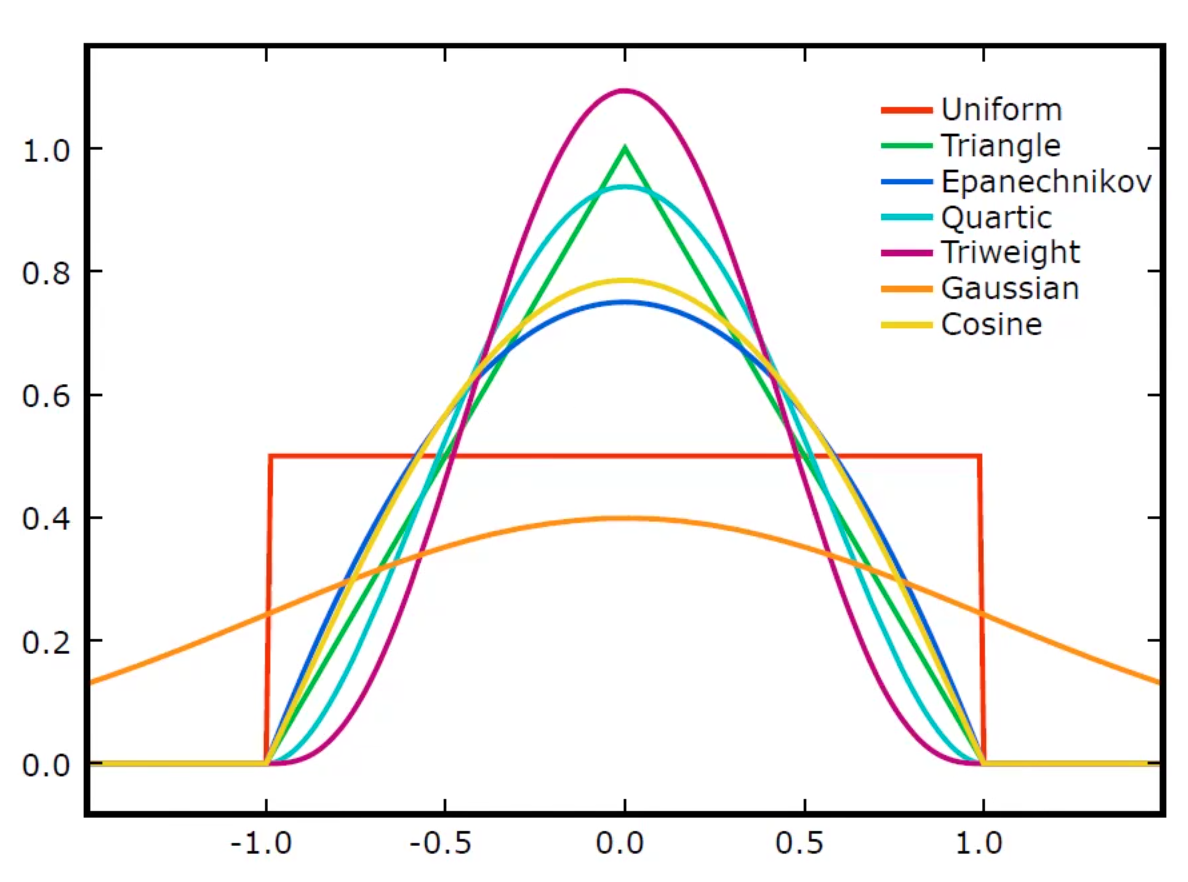
\includegraphics[width=0.8\textwidth]{Images/ml_kernel_functions}
    \end{figure}\noindent
    (Какие-то они неубывающие. А нифига, убывающие, потому что нас интересует значение функции только на $u\geqslant0$.)\\
    Так вот, если $Pr([a;b])$~--- мера вероятности на $[a;b]$, то
    \[
    p(x)=\lim\limits_{h\to\infty}\frac1{2h}Pr([x-h;x+h])
    \]
    Хотелось бы восстанавливать плотность распределения так. Тогда эмпирическая оценка (с окном шириной $h$):
    \[
    \widehat{p_h(x)}=\frac1{2nh}\sum\limits_{i=1}^n[|x-x_i|<h]
    \]
    Так вот, сюда можно всунуть ядерную функцию $K$ и получить оценку Парзена~--- Розенблатта (с окном шириной $h$):
    \[
    \widehat{p_h(x)}=\frac1{2nh}\sum\limits_{i=1}^nK\left(\frac{|x-x_i|}h\right)
    \]
    И суть в то, что $\widehat{p_h(x)}$ сходится к $p(x)$.\\
    Как обобщить это до многомерного случая? Если объекты описываются $m$ вещественными признаками $f_j\colon X\to\mathbb R$, то так:
    \[
    \widehat{p_h(x)}=\frac1n\sum\limits_{i=1}^n\prod\limits_{j=1}^m\frac1{h_j}K\left(\frac{f_j(x)-f_j(x_i)}{h_j}\right)
    \]
    Если же $X$~--- метрическое пространство с мерой расстояния $\rho$, то
    \[
    \widehat{p_h(x)}=\frac1{nV(h)}\sum\limits_{i=1}^n\prod\limits_{j=1}^m\frac1{h_j}K\left(\frac{\rho(x;x_i)}h\right)
    \]
    А $V(h)=\int_XK\left(\frac{\rho(x;x_i)}h\right)~\mathrm dx$~--- множитель нормализации. Но у нас, простите, функции ядерные, поэтому это тупо $\frac12$.\\
    Но то в непрерывном случае. А в дискретном
    \[
    \begin{aligned}
        a(u;\scriptD_{\mathrm{train}};{\color{red}h};K)&=\operatorname*{argmax}_{y\in Y}\sum\limits_{i=1}^{|\scriptD_{\mathrm{train}}|}\left[y(x_{u,i})-y\right]K\left(\frac{\rho(u;x_{(u,i)})}{\color{red}h}\right)\\
        a(u;\scriptD_{\mathrm{train}};{\color{red}k};K)&=\operatorname*{argmax}_{y\in Y}\sum\limits_{i=1}^{|\scriptD_{\mathrm{train}}|}\left[y(x_{u,i})-y\right]K\left(\frac{\rho(u;x_{(u,i)})}{\color{red}\rho(u;x_{(u,k+1)})}\right)
    \end{aligned}
    \]
    Верхнее~--- с фиксированной шириной окна, нижнее~--- с нефиксированной.\\
    Сверху мы фактически мы строим шар радиуса $h$ вокруг нашего объекта. Все объекты вне его нас не интересуют,, а внутри мы присваиваем объектам веса в зависимости от $K$.
    \begin{figure}[H]
        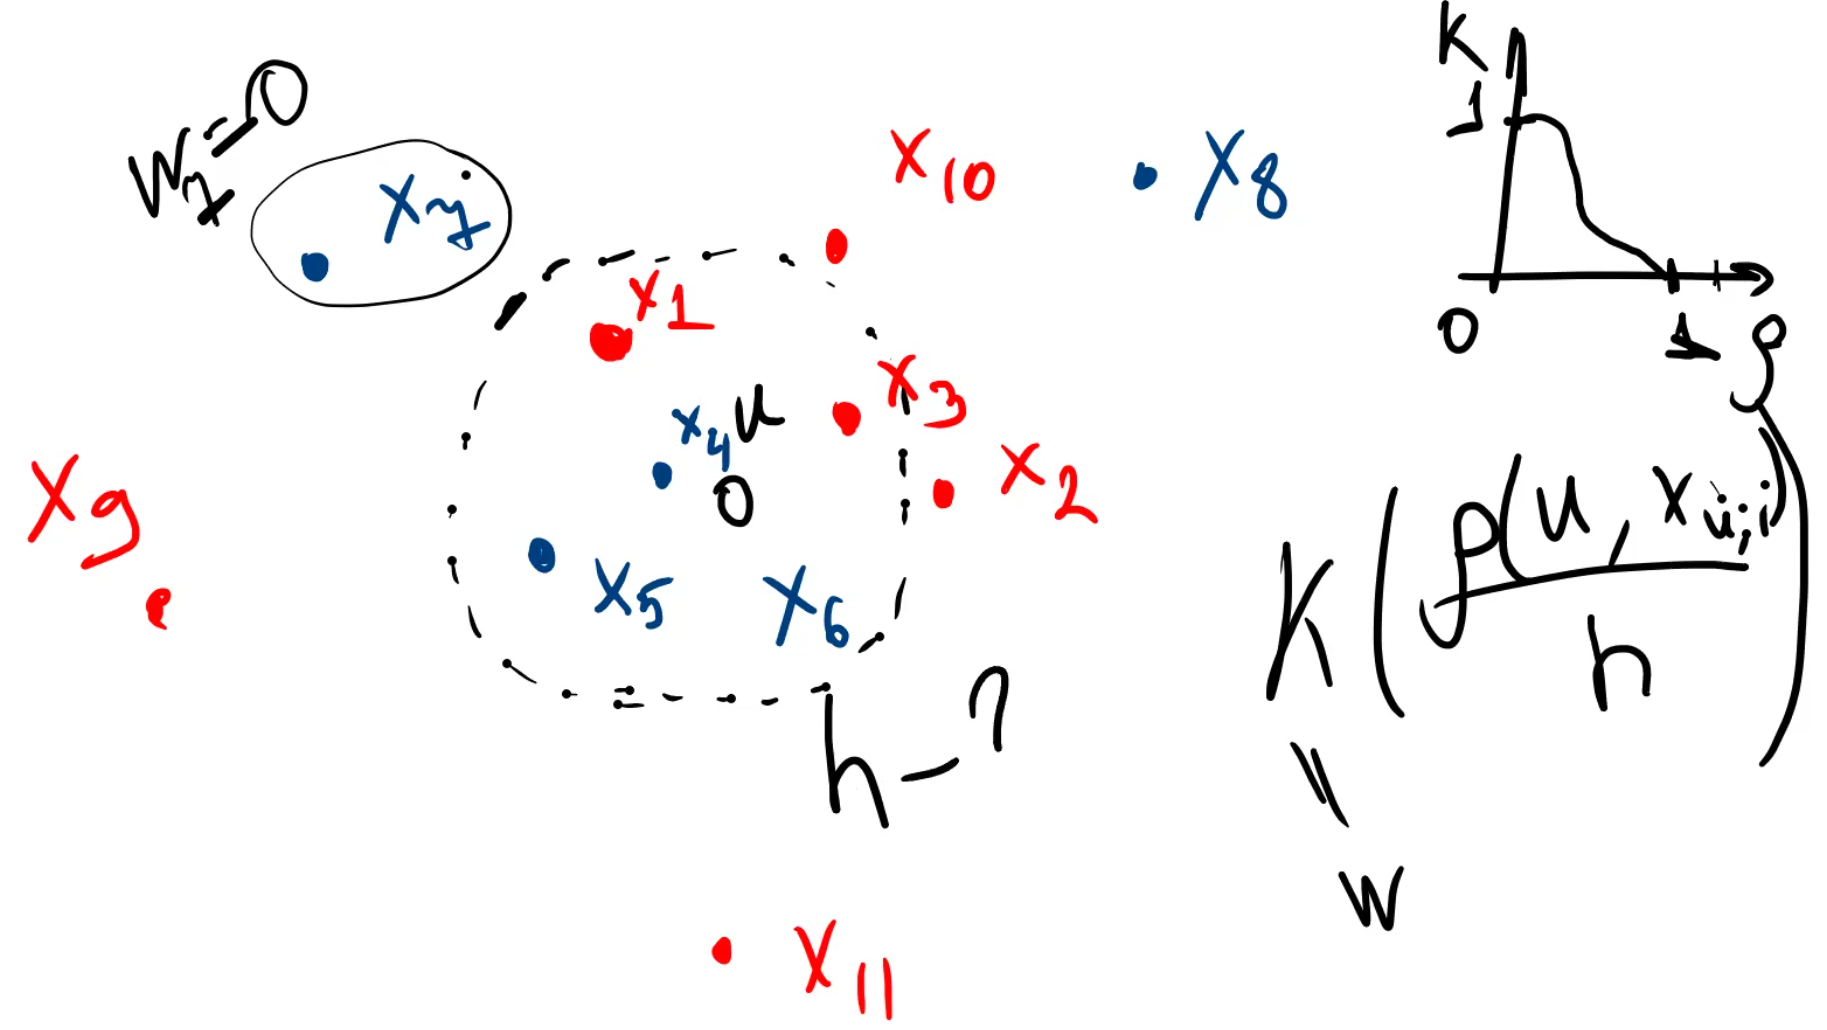
\includegraphics[width=0.8\textwidth]{Images/ml_knn-1}
    \end{figure}
    Но вопрос: как определить $h$? Для этого и есть нефиксированная ширина окна: берём до $k+1$-го соседа. То есть чтобы влияли $k$ ближайших соседей.
    \paragraph{Непараметрическая регрессия.}
    Всё выше было про классификацию, а что про регрессию? Идея схожая: будем рассматривать такие решения, что они в некоторой области $u$ константны. Тогда
    \[
    \scriptL(\theta)=\sum\limits_{i=1}^{|\scriptD_{\mathrm{train}}|}w_{(i,u)}(\theta-y(x_i))^2
    \]
    Если аналитически решать минимизацию $\scriptL$ относительно $\theta$, получится средневзвешенное.
    \begin{figure}[H]
        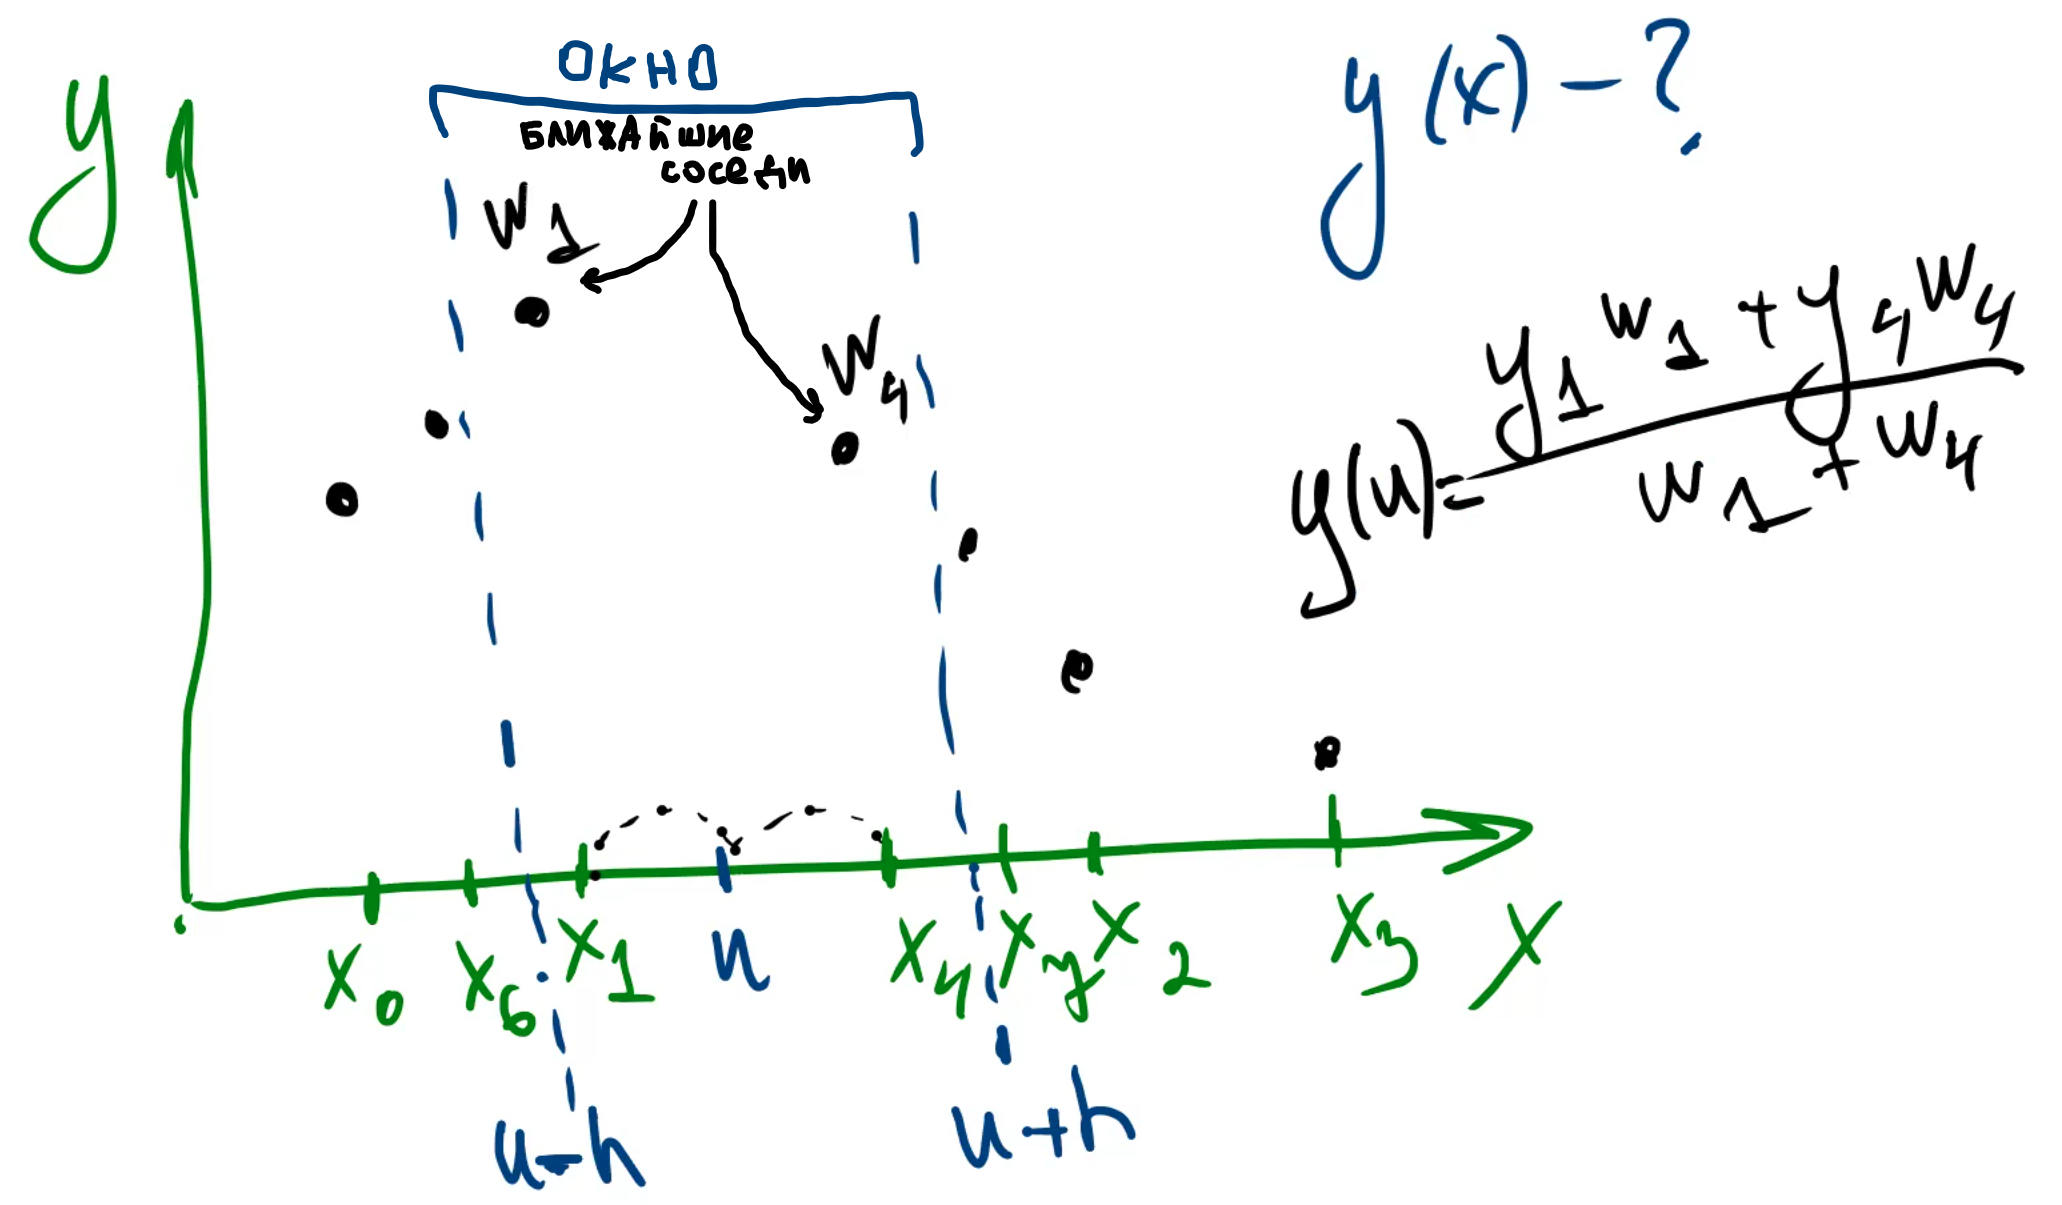
\includegraphics[width=0.8\textwidth]{Images/ml_knn-2}
    \end{figure}\noindent
    Тогда ядерное сглаживание Надарая~--- Ватсона:
    \[
    a_{\mathrm{NPR}}(u;\scriptD_{\mathrm{train}})=\dfrac{\sum\limits_{x_i\in\scriptD_{\mathrm{train}}}y_iK\left(\frac{\rho(x_i;u)}h\right)}{\sum\limits_{x_i\in\scriptD_{\mathrm{train}}}K\left(\frac{\rho(x_i;u)}h\right)}
    \]
    Тут с фиксированным окном, точно так же можно сделать и с нефиксированным.\\
    Теорема (кажется, Новикова). Пусть
    \begin{itemize}
        \item $\scriptD_{\mathrm{train}}$~--- выборка, распределённая по $p(x,y)$.
        \item $K$~--- такая ядерная функция, что $\int\limits_0^{+\infty}K(r)~\mathrm dr<\infty$ и $\lim\limits_{r\to\infty}rK(r)=0$.
        \item $\forall x\in X.\;E(y^2\mid x)<\infty$.
        \item $\lim\limits_{i\to\infty}h_i=0$, $\lim\limits_{i\to\infty}ih_i=\infty$
    \end{itemize}
    Тогда алгоритм непараметрической регрессии (по схеме Надарая~--- Ватсона) стремятся к $E(y\mid x)$ по вероятности в любой точке $x\in X$, где $E(y\mid x)$, $p(x)$, $D(y\mid x)$ непрерывны и $p(x)>0$. 
    \paragraph{Анализ всего вышеперечисленного.}
    \begin{itemize}
        \item Теоретически неравенство треугольника не нужно.
        \item Модельность метода зависит от структуры данных для хранения ближайших соседей.
        \item k-NN~--- регрессия с one-hot-преобразованием.
        \item Выбор функции ядра влияет на гладкость функции потерь, а на итоговое качество обычно влияет не так сильно.
        \item Выбор $h$ либо $k$ влияет на качество приближения.
        \item Чем больше $h$ либо $k$, тем меньше сложность модели (в крайнем случае $k=n$ алгоритм получается тождественен наивному). Вообще есть эвристика, что количество соседей выше $\sqrt n$ использовать не не надо.
    \end{itemize}
    \paragraph{Реализация.}
    Чтобы это всё быстро (хоть и приближённо) работало используется такая штука, как k-d-дерево или его аналоги.
    \paragraph{Связанные задачи.}
    \begin{itemize}
        \item Few-shot (one-shot) learning. Мало примеров, много классов, мало примеров каждого класса, причём множество классов может меняться. Основная задача (классификация)~--- 1-NN, подзадача~--- выделение признаков (строим пространство, в котором будет вычисляться расстояние). Впрочем, сейчас есть более нормальные методы.
        \item Непараметрическая генерация объектов. Берём точку $a$, смотрим $k$ ближайших точек её класса, выбираем одну, случайно выбираем точку на $(a;b)$, кидаем точку между ними с тем же классом.
        \item Поиск связей Томека. У нас могут быть близкие пары объектов разного класса (называются такие связями Томека). Если мы такое нашли, можно удалить оба, можно удалить объект мажоритарного класса, или можно объекту мажоритарного класса поменять метку. Утверждается, что мы немного восстановим компактность.
        \item LOWESS. Вместо удаления объектов их можно учитывать с меньшим локальным весом:
        \[
        w_i=K(y(x_i)-a(x_i,\scriptD_{\mathrm{train}}\setminus\{x_i\}))
        \]
        Функция ядра может отличаться от таковой в $a$, если что. Сам же $a$ может теоретически быть любым алгоритмом, но обычно используют kNN.\\
        Как такое применять для классификации? Например вот так. У нас kNN же не делает честную классификацию, он возвращает вектор вероятностей. Давайте тогда в качестве весов брать
        \[
        w_i=K\left(\|y(x_i)-a(x_i,\scriptD_{\mathrm{train}}\setminus\{x_i\})\|\right)
        \]
        Тут считается, что $y(x_i)$~--- вектор, у которого везде нули, кроме одного места, где правильный класс, а $a$ возвращает вектор вероятностей. \textit{[Про это говорится в конце лекции по Байесовским методам.]}
    \end{itemize}    
    \section{Линейные модели.}
    \paragraph{Детально о нормализации.}
    Нормализовать надо так. Сначала надо центрировать датасет (т.е. сделать так, чтобы матожидание было равно нулю). Потом их надо декоррелировать (чтобы корреляции между признаками не было), и потом нормализовать. Как декоррелировать? Посчитаем ковариационную матрицу:
    \[
    \Sigma=\frac1NX^{\mathsf T}X
    \]
    Напоминание: $\operatorname{cov}(X,Y)=\Expected[(X-\Expected X)(Y-\Expected Y)^{\mathsf T}]$.\\
    И нам нужно взять
    \[
    \widehat X=X\times\sigma^{-\frac12}
    \]
    После декорреляции наш датасет будет эллипсом, и его можно примерно нормальным распределением считать.\\
    Вспомним многомерное нормальное распределение. Плотность такая:
    \[
    f_{\mu,\Sigma}=\frac{\exp\left(-\frac12(x-\mu)^{\mathsf T}\Sigma^{-1}(x-\mu)\right)}{\sqrt{(2\pi)^k|\Sigma|}}
    \]
    А чтобы сгенерировать точку, надо представить $\Sigma=A^{\mathsf T}A$, и после этого сгенерировать вектор $z$, где $z_i$ генерируется по одномерному нормальному распределению $\operatorname{N}(0,1)$. Тогда наша точка~--- это $zA+\mu$.
    \subparagraph{Теорема о сингулярном разложении.}
    Существует теорема, утверждающая, что любая матрица $F$ размера $n\times m$ может быть представлена в виде сингулярного (оно же SVD-)разложения $F=VDU^{\mathsf T}$, где
    \begin{itemize}
        \item $V$ имеет размер $n\times m$, $V^{\mathsf T}V=E_m$, столбцы $V$~--- собственные векторы $FF^{\mathsf T}$.
        \item $D$ имеет размер $m\times m$, диагональная матрица, состоящая из корней собственных чисел $F^{\mathsf T}F$. Они называются сингулярными числами.
        \item $U$ имеет размер $m\times m$, $U^{\mathsf T}U=E_m$, столбцы $U$~--- собственные векторы $F^{\mathsf T}F$.
    \end{itemize}
    В чём метод? В том, что мы хотим спроецировать наши векторы на другое пространство. Тогда $V$~--- как объекты соответствуют базисным векторам, $U$~--- как признаки соответствуют базисным векторам, а $D$~--- важность каждого базисного вектора.
    \subparagraph{Метод главных компонент.}
    \[
    X=VDU^{\mathsf T}
    \]
    Тогда
    \[
    \Sigma^{\frac12}=U^{\mathsf T}\frac Dn
    \]
    \paragraph{Линейная регрессия.}
    Наша модель выглядит так:
    \[
    f(x;\theta)=\sum\limits_{j=1}^m\theta_jf_j(x)
    \]
    Где $\theta$~--- вектор параметров и вектора признаков $f(x)$. То есть для каждого признака есть параметр.\\
    Такую функцию надо построить (найдя $\theta$). Введём матричные обозначения.
    \[
    F=\matr{
        f_1(x_1) & \cdots & f_m(x_1)\\
        \vdots & \ddots & \vdots\\
        f_1(x_n) & \cdots & f_m(x_n)
    }
    \qquad
    y=\matr{y_1\\\vdots\\y_n}
    \qquad
    \theta=\matr{\theta_1\\\vdots\\\theta_n}
    \]
    Тут $F$~--- по сути наши данные, $y$~--- наши ответы, а $\theta$ нужно найти. Как его найти?\\
    Посмотрим на функцию ошибки в матричной норме
    \[
    \scriptL(\theta,\scriptD)=\|F\theta-y\|^2
    \]
    Это надо минимизировать по $\theta$.\\
    Возьмём производную и приравняем нулю:
    \[
    \frac{\partial\scriptL}{\partial\theta}=2F^{\mathsf T}(F\theta-y)=0
    \]
    Решение у этого такое:
    \[
    \theta^*=(F^{\mathsf T}F)^{-1}F^{\mathsf T}y
    \]
    Вообще матрица $(F^{\mathsf T}F)^{-1}F^{\mathsf T}$ называется псевдообратной (или же обратным преобразованием Мура~--- Пенроуза) и обозначается $F^+$. Спойлер: найти его явно трудно, долго и непрактично. Поэтому воспользуемся SVD-разложением:
    \[
    F^+=(UDV^{\mathsf T}VDU^{\mathsf T})^{-1}UDV^{\mathsf T}=UD^{-1}V^{\mathsf T}=\sum\limits_{j=1}^m\frac1{\sqrt{\lambda_j}}u_jv_j^{\mathsf T}
    \]
    \[
    \theta^*=F^+y=\sum\limits_{j=1}^m\frac1{\sqrt{\lambda_j}}u_j(v_j^{\mathsf T}y)
    \]
    Итого нам надо только собственные вектора найти, и всё будет хорошо.\\
    Ещё в конце нам понадобится считать $\|\theta^*\|^2$, и оно вот такую формулу имеет:
    \[
    \|\theta^*\|^2=\|D^{-1}V^{\mathsf T}y\|^2=\sum\limits_{j=1}^m\frac1{\lambda_j}(v_j^{\mathsf T}y)^2
    \]
    \subparagraph{Гребневая регуляризация.}
    Идея: чтобы избежать переобучения, будем контролировать $\|\theta^*\|^2$. Возьмём себе положительный коэффициент регуляризации $\theta$, тогда
    \[
    \scriptL_\tau(\theta)=\|F\theta-y\|^2-\tau\|\theta\|^2
    \]
    Альтернативно можно регуляризировать отдельно $\theta_j$, например, присвоив им веса $w_j$. И тогда $\tau_j=1/w_j$.\\
    Как с $\tau$ будет выглядеть формула? Ну, вот так:
    \[
    \theta^*=(F^{\mathsf T}F+\tau I_m)^{-1}F^{\mathsf T}y
    \]
    А если применить SVD, будет
    \[
    \theta^*=\sum\limits_{j=1}^m\frac{\sqrt{\lambda_j}}{\lambda_j+\tau}u_j(v_j^{\mathsf T}y)
    \qquad
    \|\theta^*\|^2=\sum\limits_{j=1}^m\frac1{\lambda_j+\tau}(v_j^{\mathsf T}y)^2
    \]
    \subparagraph{Свободный член.}
    Вообще говоря, уравнение гиперплоскости в общем виде содержит свободный член:
    \[
    f(x;\theta)=\sum\limits_{j=1}^m\theta_jf_j(x)+\theta_{m+1}
    \]
    Вместо него можно добавить признак, тождественно равный единице или минус единице. Регуляризировать его не принято: $\tau_{m+1}=0$.
    \subparagraph{Итоги.}
    Мораль проста: нам надо лишь считать сингулярное разложение. Оно в принципе очень важно много для чего. Считается, к сожалению, за $O(nm^2+m^3)$, но всяко лучше, чем искать псевдообратную.
    \paragraph{Линейная классификация.}
    Тут чуть сложнее. Для начала, мы скажем, что ограничиваемся бинарной классификацией. И считаем, что у нас классы~--- это $Y=\{1;-1\}$. А найти нам надо функцию, которая будет разделять объекты двух разных классов. То есть наши предсказания будут знаком этой функции.\\
    Как тогда мы будем строить $\theta$? Тут так легко не получится, потому что нет хорошей функции ошибки. Поэтому вместо этого сделаем функцию отступа (margin):
    \[
    M_i(\theta)=y_if(x_i;\theta)
    \]
    Если она отрицательная, объект классифицирован некорректно.\\
    Как сделать общую функцию ошибки? Можно взять количество отрицательных $M_i$. Но она такая функция не дифференцируется, поэтому экстремумы не ищутся.\\
    Поэтому вместо этого возьмём себе какую-то хорошую функцию $\scriptL$, и скажем, что
    \[
    \widetilde\scriptL(\theta)=\sum\limits_i^{|\scriptD|}\scriptL(M_i(\theta))
    \]
    Какая должна быть $\scriptL$? Гладкая, неотрицательная и невозрастающая. Примеры:
    \begin{itemize}
        \item $H(M)=(-M)_+$~--- Hebb's rule.
        \item $V(M)=(1-M)_+$~--- SVM.
        \item $L(M)=\log_2(1+e^{-M})$~--- LR.
        \item $Q(M)=(1-M^2)$~--- LDA.
        \item $S(M)=2(1+e^{M})^{-1}$~--- ANN.
        \item $E(M)=e^{-M}$~--- AdaBoost.
    \end{itemize}
    Тут исключением является LDA, но у неё правый хвост параболы выступает в роли регуляризатора. Если значение функции отступа большое, объект очень далеко от разделяющей функции. Возможно, можно было бы построить и поближе.\\
    Итого
    \[
    f(x;\theta)=\sign\left(\sum\limits_{i=1}^n\theta_if_i(x)-\theta_0\right)
    \]
    Как в итоге обучать $\theta$? Ну, теперь наш эмпирический риск гладкий, можно с ней работать, а как~--- обсудим позже.
    \paragraph{Логистическая регрессия.}
    Это про мягкую классификацию. Хотим возвращать вектор вероятностей каждого класса. Зачем? Мягкая классификация информативней и позволяет использовать более чувствительные функции ошибки. Как нам такое сделать?\\
    Используем перекрёстную энтропию:
    \[
    H(p;q)=-\sum\limits_{x\in X}p(x)\log q(x)
    \]
    Функция ошибки перекрёстной энтропии:
    \[
    \scriptL(b;x)=-\log q_{y(x)}
    \]
    Где $q_{y(x)}$~--- $y(x)$-тый элемент вектора $b(x)$.\\
    Натравим это дело на бинарную классификацию (вероятности $q_+$ и $q_-$). Эта задача называется логистической регрессией, но это не регрессия, потому что $q_+\in[0;1]$, а не $q_+\in\mathbb R$. Зато $\log\frac{q_+}{q_-}\in\mathbb R$. Это называется логит-преобразованием.\\
    Собственно, будем предсказывать $\log\frac{q_+}{1-q_+}$ при помощи линейной регрессии, тогда
    \[
    q_+=\sigma(f(x;\theta))\qquad\sigma(x)=\frac1{1+e^{-x}}
    \]
    Для логистической регрессии используется логарифмическая функция потерь:
    \[
    \scriptL(a;\scriptD)=\sum\limits_{(x,y)\in\scriptD}\ln(1+\exp(-f(x;\theta)y))
    \]
    \paragraph{Градиентный спуск.}
    Это, собственно, чем решать всё это чудо. Как мы помним, мы тут минимизируем вот это:
    \[
    \widetilde\scriptL(\theta)=\sum\limits_i^{|\scriptD|}\scriptL(M_i(\theta))=\sum\limits_i^{|\scriptD|}\scriptL(\dotprod{\theta}{x_i}y_i)
    \]
    Тогда (классический) градиентный спуск делает последовательность $\theta$. У нас есть какое-то начальное $\theta_{(0)}$, и на каждом шаге мы строим
    \[
    \theta_{(k+1)}=\theta_{(k)}-\mu\nabla\widetilde\scriptL(\theta_{(k)})
    \]
    Более детально
    \[
    \theta_{(k+1)}=\theta_{(k)}-\mu\sum\limits_i^{|\scriptD|}\scriptL'(\dotprod{\theta}{x_i}y_i)x_iy_i
    \]
    \subparagraph{Стохастический градиентный спуск.}
    Считать кучу производных за шаг~--- это долго. Поэтому люди придумали стохастический градиентный спуск. Давайте наши объекты упорядочим, и будем каждый шаг делать в направлении не суммы градиентов по всем объектам, а в направлении градиента по одному объекту, а для следующий итерации брать следующих объект.\\
    Останавливаться будем тогда, когда значения $\scriptL$ или $\theta$ будут меняться достаточно мало. В стохастическом градиентном спуске критерий остановки может сойти с ума, поэтому давайте бахнем сюда скользящее среднее:
    \[
    \scriptL_{(k+1)}=(1-\alpha)\scriptL_{(k)}+\alpha\scriptL(\dotprod{\theta}{x_i}y_i)
    \]
    Что ещё можно? Можно делать mini-batch~--- будем брать не всю выборку, как в классическом спуске, не один объект, как в стохастическом, а некоторое фиксированное количество. И тоже (как в стохастическом) менять набор на каждой итерации. Сюда тоже надо бахнуть скользящее среднее.
    \subparagraph{Проблемы.}
    Какие тут проблемы? У нас может быть производная в районе нуля, когда мы вышли на плато. А ещё можно прийти в седловую точку или в локальный минимум, где градиент нулевой. Причём это ещё и не понять никак нормально. Либо запускаться из другой точки, чтобы получить другое значение, либо использовать другие методы.
    \subparagraph{Начальные значения.}
    Как выбирать начальное значение $\theta_{(0)}$? Есть несколько эвристик.
    \begin{itemize}
        \item Можно задать нулями.
        \item Можно взять маленькие случайные значения в интервале $\left[-\frac1{2n};\frac1{2n}\right]$.
        \item Можно взять ${\theta_{(0)}}_j=\frac{\dotprod{y}{f_j}}{\dotprod{f_j}{f_j}}$.
        \item Можно взять маленькую подвыборку, погонять спуск на ней, найти какую-то точку и взять её в качестве начальной для основного спуска.
        \item А ещё можно взять предыдущую эвристику, но погонять градиентный спуск на разных подвыборках и/или из разных точек. У кого лучше получилось, того и берём в качестве начального приближения для всего датасета.
    \end{itemize}
    \subparagraph{Скорость сходимости.}
    У нас же ещё есть коэффициент $\mu$. Если взять большой, сходиться не будет. Если маленький, будет сходится медленно. И пока мы не применяем какие-то оптимизации по типу адаптивного градиента. Поэтому пока что просто обсудим эвристики:
    \begin{itemize}
        \item Можно уменьшать скорость сходимости с каждой итерацией. Это наискорейший спуск.
        \item Если мы откуда-то знаем, что мы на плато или в седловой точке, можно использовать стратегии <<выпрыгивания>>, т.е. резкого увеличения скорости сходимости.
        \item Можно использовать методы второго порядка, где такого нет.
        \item Или можно использовать средний вектор недавних шагов.
    \end{itemize}
    \subparagraph{Метод Ньютона~--- Рафсона.}
    Это к вопросу о методах второго порядка. Тут вот что делаем:
    \[
    \theta_{(k+1)}=\theta_{(k)}-\eta_k\left(\scriptL''(\theta_{(k)})\right)^{-1}\scriptL'(\theta_{(k)})
    \]
    И тут $\eta_k$ можно просто взять 1. Эта хрень не останавливается на плато и в седловых точках, но у неё есть фундаментальная беда: надо считать вторые производные. Существуют аппроксимации, но в целом в глубоких моделях методы второго порядка не используют.
    \subparagraph{Эвристика на порядок объектов.}
    На самом деле, они какого-то значительного прироста в качестве не дают. Но если хочется, вот они:
    \begin{itemize}
        \item Брать на каждом шаге предметы разных классов.
        \item Чаще брать неверно классифицированные объекты.
        \item Чаще не брать <<хорошие объекты>> ($M_i>\kappa_+$).
        \item Чаще не брать <<объекты-шумы>> ($M_i<\kappa_-$).
    \end{itemize}
    \subparagraph{Анализ.}
    Простой в реализации, легко обобщается, может динамически обучаться (это мы даже обсуждали вообще, когда говорили, что в качестве начальной точки можно выбрать результат запуска на подвыборке), поддерживает сверхмалые выборки. Однако сходится медленно (если сходится вообще), застревает где угодно, очень важно правильно подобрать эвристики для learning rate и начального значения. А ещё переобучается только так.
    \paragraph{Регуляризация.}
    Тут тоже можно применить гребневую регуляризацию, ограничив норму $\|\theta\|$ тем же способом:
    \[
    \nabla\scriptL_\tau(\theta)=\nabla\scriptL(\theta)+\tau\theta
    \qquad
    \theta_{(k+1)}=\theta_{(k)}(1-\mu)-\mu\nabla\scriptL_\tau(\theta_{(k)})=\theta_{(k)}(1-\mu\tau)-\mu\nabla\scriptL(\theta_{(k)})
    \]
    А ещё можно сделать лассо Тибширани. Давайте жёстко ограничим $\theta$:
    \[
    \sum\limits_{i=1}^n|\theta_i|\leqslant\kappa
    \]
    Для метода наименьших квадратов это тоже можно использовать, но там нет аналитического решения. Существует хорошее численное, но не о нём. С точки зрения градиентного спуска, всё хорошо. У нас
    \[
    \scriptL_\tau(\theta)=\|F\theta-y\|^2+\tau\sum_i|\theta_i|
    \]
    И это мы минимизируем.\\
    Если посмотреть на LASSO, то обнаружим, что он по сути своей неявно работает как выделение признаков, поочерёдно обнуляя веса для некоторых признаков.
    \section{Метод опорных векторов.}
    Тут мы тоже будем решать линейную классификацию, но другим способом. Идея будет такой: будем искать разделяющую поверхность, которая наиболее удалена от обоих классов. То есть по сути мы ищем разделяющую полосу, в которой не должно быть никаких объектов. И полоса должна быть максимально широкая.\\
    Когда у нас будет полоса, на обеих сторонах этой полосы будут лежать объекты (иначе полосу можно будет расширить). Тогда давайте поступим так. Мы же в итоге будем брать скалярное произведение вектора нормали и нашей точки. Так вот давайте зададим нормали такую длину, чтобы у этих самых объектов сдвинутое скалярное произведение было $\pm1$. То есть скалярное произведение в интервале $(-1;1)$ достигаться не будет.\\
    То есть у нас все отступы должны быть по не меньше единицы, а не просто положительны. А ещё когда мы так нормализуем, мы получим, что ширина полосы у нас равна $\frac2{\|w\|}$, где $w$~--- вектор нормали. Итого $\|w\|^2$ мы будем минимизировать, тем самым максимизируя ширину полосы.\\
    Итого имеем вот такую задачу:
    \[
    \left\{\begin{aligned}
        &\|w\|^2\to\min_{w,w_0}&\\
        &M_i(w,w_0)\geqslant1&i=1,\ldots,|\scriptD|
    \end{aligned}\right.
    \]
    \paragraph{Неразделимый случай.}
    А что если классы неразделимы? Тогда нужной нам гиперплоскости нет, но мы можем попытаться найти гиперплоскости с наименьшими значениями отступов для каждого объекта:
    \[
    \left\{\begin{aligned}
        &\frac12\|w\|^2+C\sum\limits_{u=1}^{|\scriptD|}\xi_i\to\min_{w,w_0,\xi}&\\
        &M_i(w,w_0)\geqslant1-\xi_i&i=1,\ldots,|\scriptD|\\
        &\xi_i\geqslant0&i=1,\ldots,|\scriptD|
    \end{aligned}\right.
    \]
    У этой задачи есть эквивалентная задача безусловной оптимизации:
    \[
    \sum\limits_{i=1}^{|\scriptD|}(1-M_i(w,w_0))_++\frac1{2C}\|w\|^2\to\min_{w,w_0}
    \]
    Здесь $(x)_+=\max(0,x)=\frac{x+|x|}2$.\\
    Как нетрудно заметить, $(1-M_i(w,w_0))_+$~--- это нижняя граница для $\xi$.\\
    Константа $C$ тут одновременно и регуляризацией выступает, и регулирует ширину полосы. Если взять маленькое $C$, будет широкая полоса, но и много нарушителей.\\
    Как решать эту хуйню? Задачей математического программирования. Это о том, что надо что-то минимизировать при некоторых условиях, где каждое условие~--- либо неравенство, либо равенство. А математического программирование будем решать так:\\
    Пусть наше математического программирование выглядит так:
    \[
    \left\{\begin{aligned}
        &f(x)\to\min&\\
        &g_i(x)\leqslant0&i=1,\ldots,m\\
        &h_j(x)=0&j=1,\ldots,k
    \end{aligned}\right.
    \]
    Составим единый лагранжиан:
    \[
    \scriptL(x,\eta,\lambda)=f(x)+\sum\limits_{i=1}^m\mu_ig_i(x)+\sum\limits_{j=1}^k\lambda_jh_j(x)
    \]
    Если мы найдём такую точку $x^*$, что $\frac{\partial\scriptL}{\partial x}(x^*,\eta,\lambda)$, то это будет точка минимума, если верны условия Каруша~--- Куна~--- Таккера:
    \[
    \left\{\begin{aligned}
        &g_i(x^*)\leqslant0\\
        &h_j(x^*)=0\\
        &\eta_i\geqslant0\\
        &\eta_ig_i=0
    \end{aligned}\right.
    \]
    Ну, у нас и так задача математического программирования, давайте составим лагранжиан:
    \[
    \scriptL(w,w_0,\xi,\alpha,\beta)=\frac12\|w\|^2-\sum\limits_{i=1}^{|\scriptD|}\alpha_i(M_i(w,w_0)-1)-\sum\limits_{j=1}^{|\scriptD|}\xi_j(\alpha_j+\beta_j-C)
    \]
    А условия минимума:
    \[
    \left\{\begin{aligned}
        &\frac{\partial\scriptL}{\partial w}=0\\
        &\frac{\partial\scriptL}{\partial w_0}=0\\
        &\frac{\partial\scriptL}{\partial\xi}=0\\
        &\xi_i\geqslant0\\
        &\alpha_i\geqslant0\\
        &\beta_i\geqslant0\\
        &\alpha_i=0\lor M_i(w,w_0)=1-\xi_i\\
        &\beta_i=0\lor\xi_i=0\\
    \end{aligned}\right.
    \]
    Отсюда можно разделить объекты на три группы:
    \begin{itemize}
        \item $\alpha_i=0$, $\beta_i=C$, $\xi_i=0$, $M_i>1$~--- периферийный объект.
        \item $0<\alpha_i<C$, $0<\beta_i<C$, $\xi_i=0$, $M_i=1$~--- опорный пограничный объект.
        \item $\alpha_i=C$, $\beta_i=0$, $\xi_i>0$, $M_i<1$~--- опорный нарушитель.
    \end{itemize}
    Нас интересуют объекты второй и третьей группы~--- т.н. опорные объекты. То есть такие, у которых $\alpha_i\neq0$.\\
    Итак, если брать производную по $w$ и подставлять $w=\sum\limits_{i=1}^{|\scriptD|}\alpha_iy_ix_i$, $x_0=\dotprod{w}{x_i}-y_i$, то получим мы, что
    \[
    -\scriptL(\alpha)=-\sum\limits_{i=1}^{|\scriptD|}\alpha_i+\frac12\sum\limits_{i=1}^{|\scriptD|}\sum\limits_{j=1}^{|\scriptD|}\alpha_i\alpha_jy_iy_j\dotprod{x_i}{x_j}\to\min_\alpha
    \]
    При этом $\forall i=1,\ldots,l~0\leqslant\alpha_i\leqslant$ и $\sum\limits_{i=1}^{l}\alpha_iy_i=0$.\\
    А линейный классификатор выглядит так:
    \[
    a(x)=\sign\left(\sum\limits_{i=1}^{|\scriptD|}\alpha_iy_i\dotprod{x_i}{x}-w_0\right)
    \]
    Примечания: несмотря на то, что тут сумма по всем объектам, всё не так плохо, потому что опорных из них будет не очень много.\\
    Тут можно остановится на этом и делать градиентный спуск, как-нибудь исправляя вектора, чтобы условия выполнялись. Но мы сейчас другим заниматься будем.
    \subparagraph{SMO.}
    В чём алгоритм? Берём каждый раз пару объектов. У них есть $\alpha_i$ и $\alpha_j$. Пусть они одного класса. Тогда если мы увеличим $\alpha_i$ на $k$, то $\alpha_j$ придётся уменьшить на $k$. При этом надо следить за тем, чтобы $\alpha_i$ и $\alpha_j$ были от нуля до $C$, а ещё за тем, чтобы целевая функция уменьшалась. Если классы разные, то к обоим $\alpha$ бы будем прибавлять $k$.\\
    Так вот, SMO заключается в том, чтобы брать $k=\alpha_i-\alpha_j$, если $y_i\neq y_j$, а иначе $k=\alpha_1+\alpha_2$.
    \paragraph{Ядерный трюк.}
    Интересный факт. Если оставить запись функции и классификатора в том виде, в котором они у нас записаны, мы увидим, что и при обучении, и при предсказании мы взаимодействуем с соседями при помощи скалярного произведения.\\
    Зачем нам это? А вот. У нас может быть выборка, которая никак нормально не разделяется. И мы хотим найти неявное отображение в многомерное пространство, в котором точки будут линейно разделимы. И поэтому вместо скалярного произведения мы будем использовать ядро, которое является скалярным произведением в неявно заданном пространстве. Почему именно так, а не с явным переводом точек в новое пространство? Потому что переход в новое пространство может быть дорогим, дороже, чем просто вычислить ядро.\\
    Итак, ядерной функцией называется $K\colon X\times X\to\mathbb R$, если её можно представить как $K(x,x')=\dotprod{\psi(x)}{psi(x')}$, где $\psi\colon X\to H$, $H$~--- пространство со скалярным произведением. Но нам важно не это. Функция является ядерной, если она симметрична и для любой функции $g\colon X\to\mathbb R$
    \[
    \int_X\int_XK(x,x')g(x)g(x')~\mathrm dx~\mathrm dx'\geqslant0
    \]
    На практике нужно нам, впрочем, не это, а положительная определённость матрицы Грама (на наших объектах).\\
    Примеры:
    \begin{itemize}
        \item $\dotprod{x}{x'}^d$. Тут можно явно узнать $H$~--- это будет пространство всех многочленов, у которых каждая степень одночлена равна $d$. И это скалярное произведение в нём.
        \item $(\dotprod{x}{x'}+1)^d$. Это пространство всех многочленов с одночленами степени меньше либо равной $d$.
        \item $\sigma(\dotprod{x}{x'})$. Эта штука в нейронных сетях используется.
        \item $\exp(-\beta\|x-x'\|^2)$.
    \end{itemize}
    Если этого не хватает, что делать? Ну, можно новые ядра придумывать:
    \begin{itemize}
        \item Константа 1~--- функция ядра.
        \item Произведение ядер~--- ядро.
        \item Если $\psi\colon X\to\mathbb R$, то $\psi(x)\psi(x')$~--- ядро.
        \item Линейная комбинация ядер~--- ядро.
        \item Если $\phi\colon X\to\mathbb X$ и $K$~--- ядро, то $K(\phi(x),\phi(x'))$~--- ядро.
        \item Если $s\colon X\times X\to\mathbb R$~--- симметричная и интегрируемая, то $\int_Xs(x,z)s(x',z)~\mathrm dz$~--- ядро.
    \end{itemize}
    \paragraph{Итог.}
    Идейно~--- алгоритм шедевральный, разделяешь любой  поверхностью~--- радуешься. Ещё и быстро, потому что опорных векторов немного. На практике удачи подобрать $C$ и ядро. А ещё алгоритм чувствителен к шуму (потому что шум может поменять то, какие вектора у нас опорные). И признаки выбирать нельзя.
    \paragraph{Связанные задачи.}
    Во-первых, можно делать другие функции регуляризации. Например, вектор релевантности:
    \[
    \frac12\sum\limits_{i=1}^{|\scriptD|}\left(\lambda_i+\frac{\alpha_i^2}{\lambda_i}\right)
    \]
    Или LASSO SVM:
    \[
    \mu\sum\limits_{i=1}^{|\scriptD|}|w_i|
    \]
    Или машина опорных признаков:
    \[
    \sum\limits_{i=1}^{|\scriptD|}R_\mu(w_i)\qquad R_\mu(w_i)=\begin{cases}
        2\mu|w_i| & |w_i|<\mu\\
        \mu^2+w_i^2 & \mathrm{otherwise}
    \end{cases}
    \]
    В последней $\mu$ называется параметром селективности. И эта штука может выбирать признаки.\\
    Ещё можно решать задачу регрессии опорными векторами. Идея будет схожая, но там будет требоваться, чтобы точки наоборот лежали внутри полосы.\\
    Можно обучаться на привилегированных данных. Тогда, если привилегированны данные обозначаются со звёздочкой, то наша задача будет выглядеть так:
    \[
    \left\{\begin{aligned}
        &\frac12(\dotprod{w}{w}+\gamma\dotprod{w^*}{w^*})+C\sum(\dotprod{w^*}{x_i^*}-w_0^*)\to\min\\
        &y_i(\dotprod{w}{x_i}-w_0)\geqslant1-(\dotprod{w^*}{x_i^*}-w_0^*)
        &\dotprod{w^*}{x_i^*}-w_0\geqslant0
    \end{aligned}\right.
    \]
    Можно и для частично размеченных данных решать задачу. Просто функция потерь содержит и расстояние до неразмеченных объектов тоже. Потому что по задумке неразмеченные объекты тоже не должны попадать в полосу. Тут, правда, получается невыпуклая оптимизация. Поэтому если вы не знаете, как с этим жить, придётся использовать сглаживание или сделать себе верхнюю оценку и разбить на несколько задач выпуклой оптимизации.\\
    А ещё можно one-class SVM, который используется для поиска аномалий. Тут мы пытаемся засунуть объекты в окружность, а нарушители будут вне её. И ещё у нас будет проекция в пространство большей размерности, которая их в окружность и засунет.
    \section{Байесовские методы и вероятностная классификация.}
    \paragraph{Формула Байеса.}
    Мы знаем, что
    \[
    p(A|B)=\frac{p(A)p(B|A)}{p(B)}=\frac{p(A\cap B)}{p(B)}=\frac{p(A)p(B|A)}{\sum\limits_ip(A_i)p(B|A_i)}
    \]
    Пример: если некоторой болезнью болеет 0.5\% населения, и есть тест, который даёт один процент false-positive ошибок и один процент false-negative, то если тест был положительным, человек болеет с вероятностью
    \[
    p(d=1|t=1)=\frac{p(t=1|d=1)p(d=1)}{p(t=1|d=1)p(d=1)+p(t=1|d=0)p(d=0)}=\frac{0.99\times 0.005}{0.99\times 0.005+0.01\times 0.995}\approx0.33
    \]
    Чтобы это понять интуитивно, запишем матрицу неточностей. Пусть у нас есть 20000 человек. Тогда из них болеть будет 100, а остальные будут здоровыми. При этом для этих ста человек тест нам скажет, что 99 из них больные, а один здоровый, а из 19900 оставшихся тест скажет, что у нас 199 больных:
    \[
    \mathrm{CM}=\left[\begin{matrix}99&1\\199&19701\end{matrix}\right]
    \]
    И вот если нам тест говорит, что человек болен, то это левый столбец, и как видно по матрице, реально он болен с вероятностью примерно треть.
    \paragraph{Оценка апостериорного максимума.}
    Зачем нам собственно это нужно? А пусть у нас не функция $y(x)$, а некоторая совместная вероятность $p(x,y)$. И тогда наши данные~--- это независимые наблюдения одного и того же распределения.\\
    Тогда наш риск
    \[
    R(a)=\sum\limits_{y\in Y}\lambda_y\int_{a(x)\neq y}p(x,y)~\mathrm dx
    \]
    Где $\lambda_y$~--- вес класса $y$. То, насколько плохо, что мы именно класс $y$ плохо классифицируем. Эти числа обычно определяются экспертно: вам их прямо с задачей дают. Типа <<минимизируйте ошибку с вот такими весами>>.\\
    Как это пользоваться? Пусть у нас есть объект и есть класс. И нам надо посчитать, что объект принадлежит этому классу. То есть найти нам надо $p(y|x)$, и мы знаем, что $p(x)p(y|x)=p(y)p(x|y)$.
    \begin{itemize}
        \item $p(y)$~--- априорная вероятность класса $y$.
        \item $p(x|y)$~--- правдоподобие (likehood) класса $y$.
        \item $p(y|x)$~--- апостериорная вероятность класса $y$.
    \end{itemize}
    Нам надо лишь найти класс с наибольшей вероятностью. Поскольку $p(x)$ не зависит от класса, на него забьём, и будем максимизировать $p(y)p(x|y)$. Это называется оценкой апостериорного максимума (maximum aposteriori probability, MAP). Даже если нам надо получить вектор вероятностей, мы всё равно не будем считать $p(x)$, потому что это сложно. Вместо этого мы посчитаем $p(y)p(x|y)$ для каждого класса, после чего поделим на сумму полученных значений.\\
    Вспоминая о том, что у нас есть $\lambda_y$, если мы хотим достичь минимального среднего риска, нам нужен классификатор $\operatorname*{argmax}_{y\in Y}\lambda_yp(y)p(x|y)$. Это оптимальный байесовский классификатор, а его риск~--- байесовским риском.\\
    Разделяющая поверхность для двух классов $y_1$ и $y_2$~--- это множество точек, для которых $\lambda_{y_1}p(y_1)p(x|y_1)=\lambda_{y_2}p(y_2)p(x|y_2)$. Из интересного, если объекты эти классов~--- гауссианы с одинаковой матрицей ковариаций и одинаковым весом, то это просто линия/плоскость/гиперплоскость. И наш метод превращается в расстояния до ближайшего центроида (в каждом классе находим центр, дальше классифицируем исходя из ближайшего центра). Получается красивая диаграмма Вороного.
    \paragraph{Оценка плотности вероятности. Наивный байесовский классификатор.}
    Наивный байесовский классификатор: $p(x|y)$ оценивается независимо по каким-то признакам:
    \[p(x|y)=\prod\limits_jp(x_j|y)\]
    Например, если у нас есть текст (наш $x$~--- это текст), то мы пилим его на слова, и отдельно рассматриваем $p(x_j|y)$ (где $x_j$~--- встретилось ли слово). Нам нужно очень много текстов, но сильно меньше, если бы мы пытались посчитать $p(x|y)$ не наивно, где $x$~--- именно что текст, потому что тогда нам надо было текстов больше, чем комбинаций всех слов.\\
    То есть без наивности мы оцениваем вероятность встретить текст в данном классе, что сложно и нужно очень много данных. А с ней мы оцениваем отдельные слова, а вероятность текста получаем как произведение вероятностей слов.\\
    На практике эту штуку логарифмируют, чтобы иметь дело с суммой, а не произведением.\\
    Примечание. Порядок слов у нас теряется не в наивном классификаторе как таковом, а скорее в предобработке, потому что уже там мы преобразуем текст в какой-то вектор без порядка на словах. Поэтому некорректно считать, что наивный байесовский классификатор теряет порядок: порядок потеряли до него.\\
    Из интересного, в kNN мы тоже своего рода искали плотность: брали объекты данного класса из списка $k$ ближайших соседей и суммировали их веса, получая некоторый аналог правдоподобия класса $y$.
    \subparagraph{Байесовская сетью.}
    Что делают люди на самом деле? Люди используют экспертные знания. Типа если мы хотим узнать что-нибудь про рак, то мы знаем, что курение и загрязнение окружающей среды влияют на него, и при этом наличие рака влияет на результат рентгена лёгких. И нам дают информацию о том, какие признаки от каких зависят и как. И в итоге у нас получается такая сеточка
    \begin{figure}[H]
        \begin{tikzpicture}[node distance=20mm, state/.style={draw,ellipse}]
            \node[state] (C) {Cancer};
            \node[state, above left of=C] (P) {Pollution};
            \node[state, above right of=C] (S) {Smoker};
            \node[state, below left of=C] (X) {XRay};
            \node[state, below right of=C] (D) {Dyspnoea};
            \draw[->] (P) -- (C);
            \draw[->] (S) -- (C);
            \draw[->] (C) -- (X);
            \draw[->] (C) -- (D);
        \end{tikzpicture}
    \end{figure}\noindent
    И нам умные люди уже дали информацию о том, какая зависимость на какой стрелке написана. И после этого мы можем определить любой принак целевым, и оценить, как он зависит от остальных.\\
    \subparagraph{Частотный метод оценки вероятности.}
    Можно применить метод максимального правдоподобия. Например, мы знаем, что у нас нечестная монетка, тогда мы смотрим на наш датасет, видим, что там $h$ раз орёл и $t$ раз решка, то мы знаем, что такое должн происходить с вероятностью $\theta^h(1-\theta)^t$ (где $\theta$~--- неизвестная нам вероятность орла). Тогда
    \[
    \frac{\mathrm dP(H=h,T=t|\theta)}{\mathrm d\theta}=-(1-\theta)^{t-1}\theta^{h-1}(t\theta+h(\theta-1))
    \]
    Это равно нулю когда $\theta=\frac h{h+t}$. Вот там и вероятность, берём и используем.\\
    В более общем же случае получаем, что $p(c_i)=\frac{\operatorname{cnt}(c_i)}{\sum_j\operatorname{cnt}(c_j)}$.\\
    Но можно и другое сделать. Давайте считать, что $\theta$~--- тоже какая-то величина и что $p(\theta)=1$. Тогда мы получим нечто другое, а именно то, что $p(H|\scriptD)=\frac{h+1}{h+t+2}$:
    \[
    p(\theta|\scriptD)=\frac{p(\theta)p(\scriptD|\theta)}{p(\scriptD)}=\frac{p(\theta)p(\scriptD|\theta)}{\int p(\theta')p(\scriptD|\theta')\mathrm d\theta'}=\frac{p(\scriptD|\theta)}{\int p(\scriptD|\theta')\mathrm d\theta'}=\frac{\theta^h(1-\theta)^t}{\int (\theta')^h(1-(\theta'))^t~\mathrm d\theta'}=\frac{\theta^h(1-\theta)^t}{B(h+1;t+1)}
    \]
    \[
    p(H|\scriptD)=\int p(H|\theta)p(\theta|\scriptD)~\mathrm d\theta=\int\theta\frac{\theta^h(1-\theta)^t}{B(h+1;t+1)}~\mathrm d\theta=\frac{B(h+2;t+1)}{B(h+1;t+1}=\frac{h+1}{h+t+2}
    \]
    Это называется аддитивным сглаживанием (оно же сглаживание Лапласа):
    \[
    p_\alpha(c_i)=\frac{\operatorname{cnt}(c_i)+\alpha}{\sum_j(\operatorname{cnt}(c_j)+\alpha)}
    \]
    Как правило, $\alpha\in(0;1)$.
    \paragraph{MSE с регуляризацией.}
    Пусть у нас есть модель $a_\theta(x)$ (без $\theta$), но данные взяты из этой модели с шумом: $y_i=a_\theta(x_i)+\varepsilon_i$, и шум распределён нормально с отклонением $\sigma$. Тогда, вот это рофел, мы получим, что метод максимального правдоподобия даст нам то же самое, что и минимизация MSE. Но если мы ещё и сделаем распределение над $\theta$, и $\theta_j$ из нормального распределения с отклонением $\sigma_j$, то мы получим $L_2$-регуляризацию. Если же брать $\theta_j$ из распределения Лапласса, получим $L_1$-регуляризацию.
    \paragraph{SoftArgMax и SoftMax.}
    Это нам понадобится в глубоком обучении. А именно хреначить классификацию градиентным спуском, сводя к регрессии. У нас была сигмоида, которая позволяла возвращать вероятности, а как делать это с множеством классов?
    \[
    \SoftArgMax(x_1;\ldots;x_k)=\left[\begin{matrix}\frac{\exp(x_1)}{\sum_j\exp(x_j)}&\cdots&\frac{\exp(x_k)}{\sum_j\exp(x_j)}\end{matrix}\right]
    \]
    По сути мы превращаем множество чисел в множество вероятностей как-то возрастающе. Тут $x_i$ называется логитом. Прикол в том, что мы теперь можем это дифференцировать:
    \[
    \frac{\partial y_i}{\partial x_j}=y_i([i=j]-y_j)
    \]
    Теоретически функция заебись. На практике если брать числа больше 750 мы получим тупо бесконечность, а если меньше -750, то ноль. И с нулём ещё можно жить как-то (хотя это тоже плохо), то с бесконечностью всё совсем херово.\\
    Чинится это при помощи вот такого свойства:
    \[
    \SoftArgMax(x_1;\ldots;x_k)=\SoftArgMax(x_1-c;\ldots;x_k-c)
    \]
    Так мы точно не сможем получить бесконечность. Но с большей вероятностью можем вернуть ноль. Чем плох ноль? А тем, что теперь мы не можем засунуть результат в перекрёстную энтропию, потому что мы будем брать логарифм нуля :(.\\
    Ещё бывает SoftArgMax с температурой:
    \[
    \frac{\exp(x_i/t)}{\sum_j\exp(x_j/t)}
    \]
    Если устремить $t$ у нулю, получится обычный $\operatorname{argmax}$, а если к бесконечности, то получится равномерное распределение.\\
    Ещё есть функция SoftMax, она же LogSumExp, суть которой в том, что логарифм суммы экспонент примерно равен максимуму:
    \[
    \SoftMax(x_1;\ldots;x_n)=\ln\left(\sum\limits_i\exp(x_i)\right)
    \]
    Тут есть проблема, что если подставить одно и то же значение много раз, то мы не получим его же, но одно полезное свойство есть:
    \[
    \SoftMax(x_1+a;\ldots;x_n+a)=\SoftMax(x_1;\ldots;x_n)+a
    \]
    Производная этого друга~--- SoftArgMax.\\
    Можно брать другие гладкие аналоги максимума, например, $\dotprod{x}{\SoftArgMax(x)}$. Она как раз возвращает свой аргумент, если засунуть его в функцию много раз, а ещё инвариантна относительно переноса, и её значение лежит между минимумом и максимумом аргументов. Но она не сохраняет монотонность :(. Если вы решаете максимизацию, это очень большая проблема. Если же вы минимизируете максимум, то она сильно лучше LogSumExp.\\
    Ещё одно интересное свойство: $\ln(\SoftArgMax_i(x))=x_i-\SoftMax(x)$. Хотим считать перекрёстную энтропию~--- вот, пожалуйста, стабильно можно вычислить, без всяких логарифмов нуля.\\
    Языковой нюанс: SoftArgMax часто неверно называют SoftMax. Более того, функция \Verb|cross_entropy| из PyTorch  не вычисляет перекрёстную энтропию, а вычисляет SoftArgMax, и от него берёт перекрёстную энтропию.\\
    Можно рассматривать SoftArgMin как SoftArgMax от минус аргумента.
    \section{Временные ряды.}
    Раньше мы рассматривали модели, где было отображение $X\to Y$. Сейчас мы поговорим про авторегрессионные задачи. По известным данным в истории, мы предсказываем будущее.\\
    Временной ряд~--- значения, которые измерятся через постоянные интервалы. Используется везде вообще. Предсказывание притока и оттока пользователей, цен на товары, торговли акциями и т.д. В последнем случае у нас не чисто ряд, но ещё и некоторые дополнительные данные, так что это мультимодальная модель, но временной ряд там тоже есть.
    \paragraph{Свойства временных рядов.}
    Временной ряд со временем деградирует, и быстро. Нам надо не только хорошо обучаться, но и быстро. И учитывать новые данные. Лучше тут работают рекуррентные нейронные сети, но они долго обучаются. Если вы раз в неделю переобучаете SARIMA, то это норм. А если у вас сложные большие модели, которые надо долго обучать, то вы проиграли.\\
    Ещё одна важная особенность временных рядов в том, что наши данные зависимы. То, что было в настоящем, скоррелировано с тем, что было в прошлом. У нас может быть глобальный тренд на повышение чего-нибудь со временем.\\
    Компоненты рядов (определения условны, их обычно формализуют на конкретном алгоритме):
    \begin{itemize}
        \item Тренд~--- плавное долгосрочное изменение уровня. Например, по годам потребление электричества в  среднем растёт (см. ниже).
        \item Сезонность~--- циклическое изменение уровня ряда с постоянным периодом. Например, видна сезонность на картинке ниже с периодом в год.
        \item Цикл~--- циклическое изменение уровня ряда с непостоянным периодом. Обычно непонятно, как этим пользоваться.
        \item Непрогнозируемая ошибка~--- хаотическая случайная компонента.
    \end{itemize}
    \begin{figure}[H]
        \includegraphics[width=.7\linewidth]{"Images/Потребление электричества по годам в Австралии"}
    \end{figure}\noindent
    Обычно алгоритмы пытаются найти цикл, и его длина является гиперпараметром.\\
    Смысл в чём? В том, что алгоритмы умеют распиливать временной ряд на тренд, сезонность, возможно, цикл, и остатки. Тренд по-простому можно посчитать как среднее в каком-то окошке, а дальше вычесть (если ряд аддитивный) либо поделить (если мультипликативный) ряд на тренд, и поискать уже там циклы и сезоны. Это всё называется \Verb|seasonal_decompose|.
    \begin{figure}[H]
        \includegraphics[width=.7\linewidth]{"Images/Цена акций Apple за 2020"}
    \end{figure}\noindent
    Виды рядов:
    \begin{itemize}
        \item Стационарный ряд~--- неизменный во времени, грубо говоря. Статистически~--- если в любой момент времени равны матожидания, дисперсии и если ковариация между равными отрезками одинакова. Как это увидеть? Матожидание растёт~--- есть тренд.
        \begin{figure}[H]
            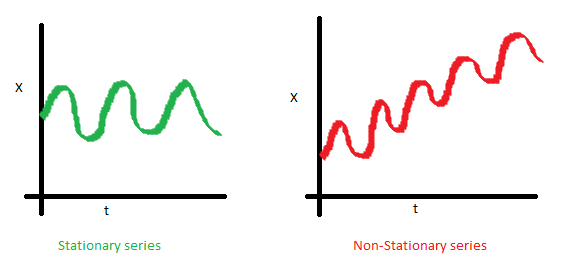
\includegraphics[width=.7\linewidth]{Images/Non-stationary_series_1}
        \end{figure}\noindent
        Дисперсия меняется~--- есть какое-то подобие сезонности, но амплитуда меняется.
        \begin{figure}[H]
            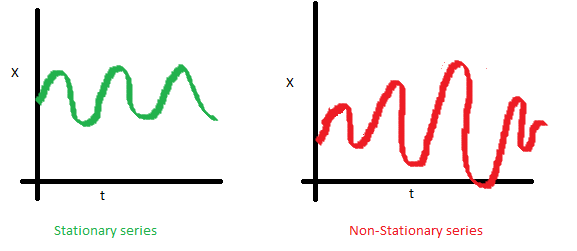
\includegraphics[width=.7\linewidth]{Images/Non-stationary_series_2}
        \end{figure}\noindent
        Ковариация разная~--- наличие цикла (но не сезона).
        \begin{figure}[H]
            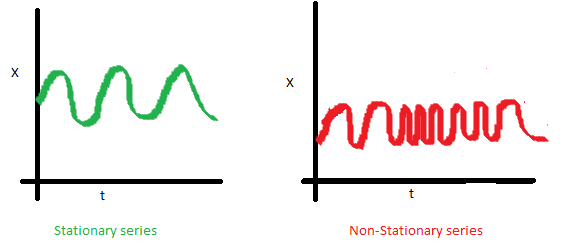
\includegraphics[width=.7\linewidth]{Images/Non-stationary_series_3}
        \end{figure}\noindent
        Такие ряды довольно легко предсказывать,, в предположении, что эти характеристики не поменяются. Помимо просмотра глазками на ряд можно провести тест Дики-Фуллера. Он, к сожалению, не гарантирует ничего, но лучше, чем ничего не проверять.\\
        Из интересного, если в нашем ряде есть тренд вида $ax+b$, можно его легко убрать, и если это единственная наша проблема, получить стационарный ряд.
        \item Интегрированный ряд. Это ряд, который при дифференцировании превращается в стационарный. Дифференцирование тут состоит в том, чтобы хранить разницы между соседними значениями вместо оригинальных. И если после нескольких дифференцирований получится стационарный, то наш ряд интегрированный.
        \item Сезонно детерминированный ряд~--- такой в котором нет случайной компоненты, и он точно описывается аналитической функцией. Сезонность можно посмотреть по автокорреляции. Это корреляция Пирсона ряда с самим собой, но сдвинутым на заданное число шагов (лагов). Если у нас в график автокорреляции в зависимости от лага сам по себе цикличен (и не лежит в статистически незначимой зоне), значит есть цикличность. А ещё этот тест может помочь вам проверить ряд на стационарность. Если с дисперсией и ожиданием всё хорошо, и все автокорреляции (кроме нескольких первых) статистически незначимы, это хороший кандидат на стационарность. Если встречаются очень редкие пики, это могут быть выбросы.
    \end{itemize}
    \paragraph{Преобразования временных рядов.}
    Можно изменить частоту измерений. Так у нас будет меньше данных, и жить может стать веселее. Это ещё называется изменением гранулярности ряда. Если нам дали много данных, мы можем рассмотреть любую гранулярность. Хотим~--- дневную, хотим~--- среднемесячные.\\
    Можно логарифмировать ряд. Если у нас монотонная дисперсия, это хорошо его стабилизирует. Есть ещё логарифмирование на стероидах~--- преобразование Бокса~--- Кокса:
    \[
    y'_t=\begin{cases}
        \ln y_t & \lambda=0\\
        (y_t^\lambda-1)/\lambda & \lambda\neq0
    \end{cases}
    \]
    Важно не забывать конвертировать ряд обратно, если забыть и посчитать ошибку для этого ряда, она будет конской. Обратно так:
    \[
    \hat y_t=\begin{cases}
        \exp y'_t & \lambda=0\\
        (\lambda y'_t+1)^{1/\lambda} & \lambda\neq0
    \end{cases}
    \]
    Очень жаль, оно не работает, если во временных рядах отрицательные значения. С этим жить понятно, как, прибавить ко всем членам константу.\\
    Дифференцирование~--- уже обсуждали, считаем попарные разности соседних элементов. Это отлично спиливает матожидание. А если ещё и много раз дифференцировать, то ещё и от сезонности избавимся.\\
    Можно захерачить FFT, но его никто не использует :) Оно только в анализе звука и речи используется, да и там его почти заменили.
    \paragraph{Экспоненциальное сглаживание.}
    Смысл простой, как в градиентном спуске было: $v_{i+1}=\alpha x_i+(1-\alpha)v_i$. Можно экспоненциально скользить чуть потруднее, например, так:
    \[
    \mathrm{level}_1=x_0\qquad\mathrm{trend}_1=x_1-x_0
    \]
    \[
    \mathrm{level}_{i+1}=\alpha\cdot x_i+(1-\alpha)\cdot(\mathrm{level}_i+\mathrm{trend}_i)\]
    \[
    \mathrm{trend}_{i+1}=\beta\cdot(\mathrm{level}_{i+1}-\mathrm{level}_i)+(1-\beta)\cdot\mathrm{trend}_i
    \]
    \[
    x_{i+1}=\mathrm{trend}_{i+1}+\mathrm{level}_{i+1}
    \]
    А можно ещё добавить сюда сезонное сглаживание, тогда получится модель Хольта~--- Уинтерса. У неё размер сезона~--- это гиперпараматр, если что. Суть всё та же, экспоненциально сглаживаем несколько компонент нашей функции.\\
    Все эти методы запаздывают за функцией и, в целом, могут что-нибудь предсказать, но весьма сомнительно.
    \paragraph{AR+MA (авторегрессия и скользящее среднее).}
    Давайте считать, что наше текущее значение зависит как-то от нескольких предыдущих:
    \[
    y_t=\alpha+\phi_1y_{t-1}+\phi_2y_{t-2}+\cdots+\phi_py_{t-p}+\epsilon_t
    \]
    Это называется авторегрессией порядка $p$.\\
    А ещё можно считать, что наше значение~--- линейная комбинация шума (из \Verb|seasonal_decompose|) на $q$ шагов назад:
    \[
    y_t=\alpha+\epsilon_t+\theta_1\epsilon_{t-1}+\cdots+\theta_q\epsilon_{t-q}
    \]
    Это модель скользящего среднего порядка $q$.\\
    Так вот, мы хотим взять комбинацию этого:
    \[
    y_t=\alpha+\phi_1y_{t-1}+\phi_2y_{t-2}+\cdots+\phi_py_{t-p}+\epsilon_t+\theta_1\epsilon_{t-1}+\cdots+\theta_q\epsilon_{t-q}
    \]
    Это ARMA порядков $p$ и $q$. Согласно теореме Вольда, любой стационарный ряд может быть описан ARMA, если правильно подобрать $p$ и $q$. Удачи доказать, что он стационарный :)\\
    Ещё модель: $\operatorname{ARIMA}(p;d;q)$~--- $d$ раз дифференцируем, применяем ARMA.\\
    SARMA~--- модификация для сезонов. Сами как-нибудь находим сезонность, после чего модифицируем ARMA так: давайте помимо $p$ и $q$ у нас будет $P$ и $Q$. И $P$ смотрит на $y_{t-s},y_{t-2s},\ldots,y_{t-Ps}$, а $Q$ смотрит на $\epsilon_{t-s},\epsilon_{t-2s},\ldots,\epsilon_{t-Qs}$. И там коэффициенты тоже свои ($\Phi$ и $\Theta$).\\
    SARIMA~--- комбинация этих двоих. Тут два дифференцирования, если что. Потенциально разное количество раз. Нынче это (и производная от ней SARIMAX)~--- самый перспективный способ предсказывать временные ряды.\\
    А ещё в таких моделях для настройки гиперпараметров используют информационный критерий Акаике (AIC), про который не рассказали ничего, кроме того, что он считается быстрее, чем полная настройка модели с текущими гиперпараметрами. И что он обычно используется в ARMA-based моделях.
    \section{Обработка текста.}
    Для начала надо текст токенизировать. Ещё для классических методов выкидывают слова, у которых у самих нет смысла. Т.е. предлоги, союзы и частицы. Они называются stop tokens. Да, выкидывать <<не>> странно, но классические методы будут лучше без него, чем с ним.\\
    Потом надо формы одного слова сделать одинаковыми. Тут либо лемматизация, либо стемминг. В первой мы приводим слова к какой-то нормальной форме (существующей), а во втором по некоторым эвристикам отбрасываем окончания и, возможно, приставки. Например, можно взять \href{http://snowball.tartarus.org/algorithms/russian/stemmer.html}{стеммер Портера}, которая на базе кучи регулярных выражений что-нибудь пытается. И получает ошибку на маленьких словах. И превращает <<которая>> в <<котор>>.\\
    Чуть более адекватным анализом занимается pymorphy3, которому мы скармливаем слово, и оно пытается понять, что это за слово. Не всегда успешно, потому что без контекста не понятно, что такое <<стали>>~--- родительный падеж от <<сталь>> или множественное число прошедшего времени от <<стать>>. По-хорошему нужно лемматизировать в контексте, но можно взять и простую эвристику~--- самое частое (т.е. первое в массиве того, что вернул pymorphy).\\
    Что после этого можно сделать? Можно скормить наши тексты в \Verb|CountVectorizer|, тут уже встроенный токенизатор, словарик и куча всего ещё. Из интересного, есть \Verb|max_df| и \Verb|min_df|~--- позволяют игнорировать слишком частые и слишком редкие слова. Слишком частые скорее всего будут аналогом stop-слов, а слишком редкие будут недоступны для понимания нашей моделью. Поскольку данные у нас разреженные, можно бахнуть байесовский классификатор. Из интересного, можно ему скормить свой токенизатор, который сделает с текстом всё, что угодно. Например, вместо настоящих слов будет давать какие-то сочетания (главное в этом случае отключить lowercase). Или который сделаем токенизацию, но на этом не остановится и лемматизирует каждое слово.\\
    Ещё есть \Verb|TfidfVectorizer|, который похож на \Verb|CountVectorizer|, у котрого основные параметры те же, и он помимо числа (а точнее, процента) встреч мы смотрим на idf~--- логарифм отношения количества документов к количеству документов, где данное слово встретилось. При помощи этого очень удобно считать перекрёстную энтропию. Смысл в том, чтобы бороться с часто встречаемыми словами, у таких слов idf будет близок к нулю.
    \paragraph{word2vec.}
    Давайте возьмём окно размера, например, 5, и по первому, второму, четвёртому и пятому словам будем предсказывать третье. Или наоборот, по слову получать 4 слова вокруг него. Первое~--- CBOW, второе~--- skip-gram.\\
    Сначала рассмотрим подход к простой памяти. У нас слова~--- это категории, которым мы сделали OHE. И мы домножаем наши слово на какую-то матрицу, мы будем извлекать её строку. Поэтому мы вообще можем сказать, что у нас есть матрица размера $d\times k$, где $k$~--- количество слов, а $d$~--- гиперпараметр, и тогда вместо OHE мы можем брать строки этой матрицы (т.е. просто все результаты OHE домножить на матрицу). Поскольку $d$ много меньше $k$, памяти будет меньше. Именно такое преобразование называется word2vec, и с помощью его уже можно решать какие-то задачи. И если правильно будет сделана матрица, получится, что $P(<<cats>>)-P(<<cat>>)+P(<<dog>>)\approx P(<<dogs>>)$.
    \paragraph{Работа с символами.}
    Для начала заметим, что можно брать пары/тройки/etc слов. Что можно, но сложно, потому что пар слов будет очень много. Но вот если мы такое преобразование будем делать символам, будет лучше. Если брать их по $n$ штук, это будет называться $n$-граммами. Но тут лучше делать немного другое преобразование: брать группы символов, которые часто встречаются вместе, и соединять их вместе. За счёт этого можно делать весьма своеобразную, но всё же токенизацию. И по итоге все токены должны встречаться примерно равновероятно. Такое называется BPE (byte pair encoding), и оно выделяет <<слова>> само, и не надо думать о том, какое брать $n$. Использовать и то, и другое можно для генерации, например.
    
\end{document}